\xsection{myblue}{Sample comparison}

\begin{frame}
  \frametitle{Comparison - \# Pandora PFOs in a
      \texorpdfstring{{$\nu\bar{\nu}H$}}{vvH} event}
  \begin{columns}[c,onlytextwidth]
  \begin{column}{0.35\textwidth}
  A shift towards higher values and more smeared out:

  $\gamma \gamma \rightarrow$low-$p_T$ hadron background now increased
  (to $\approx 1.6$ events/bunch crossing).
  \newline\newline
  \onslide<2->{The distributions of only the actual Higgs decay products are similar.}
  \end{column}
  \begin{column}{0.65\textwidth}
  \begin{tikzpicture}
    \node (img1) {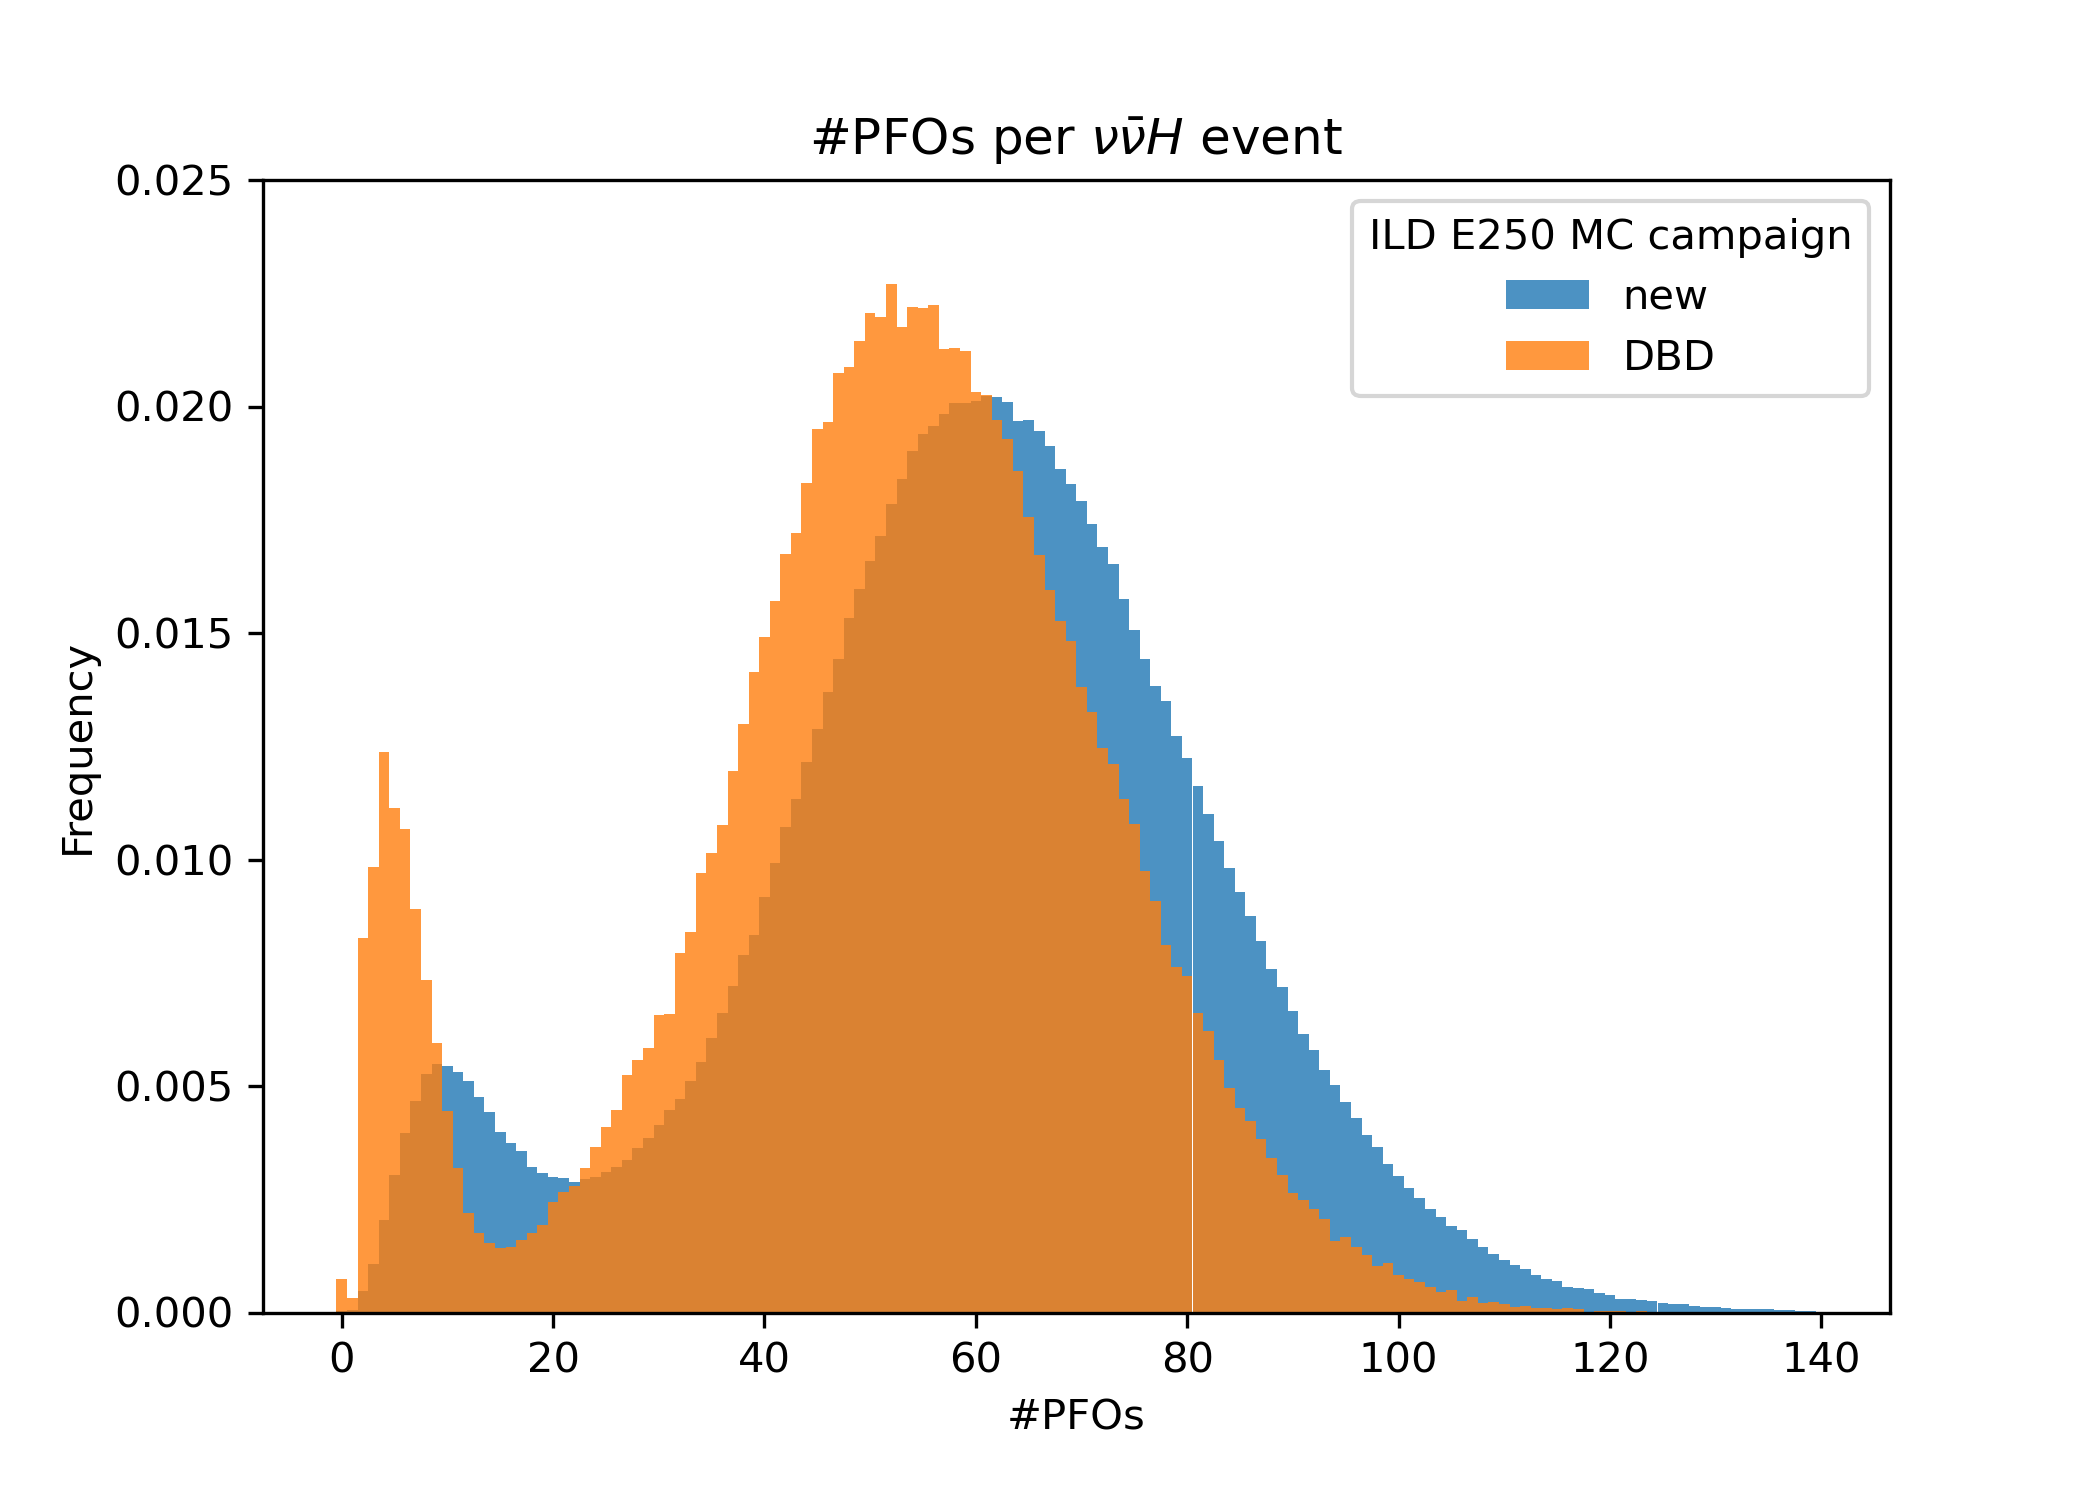
\includegraphics[height=\textheight, width=\textwidth, keepaspectratio]
        {n_pfos_full_event}};
    \node (img2) at (img1) {\only<2->{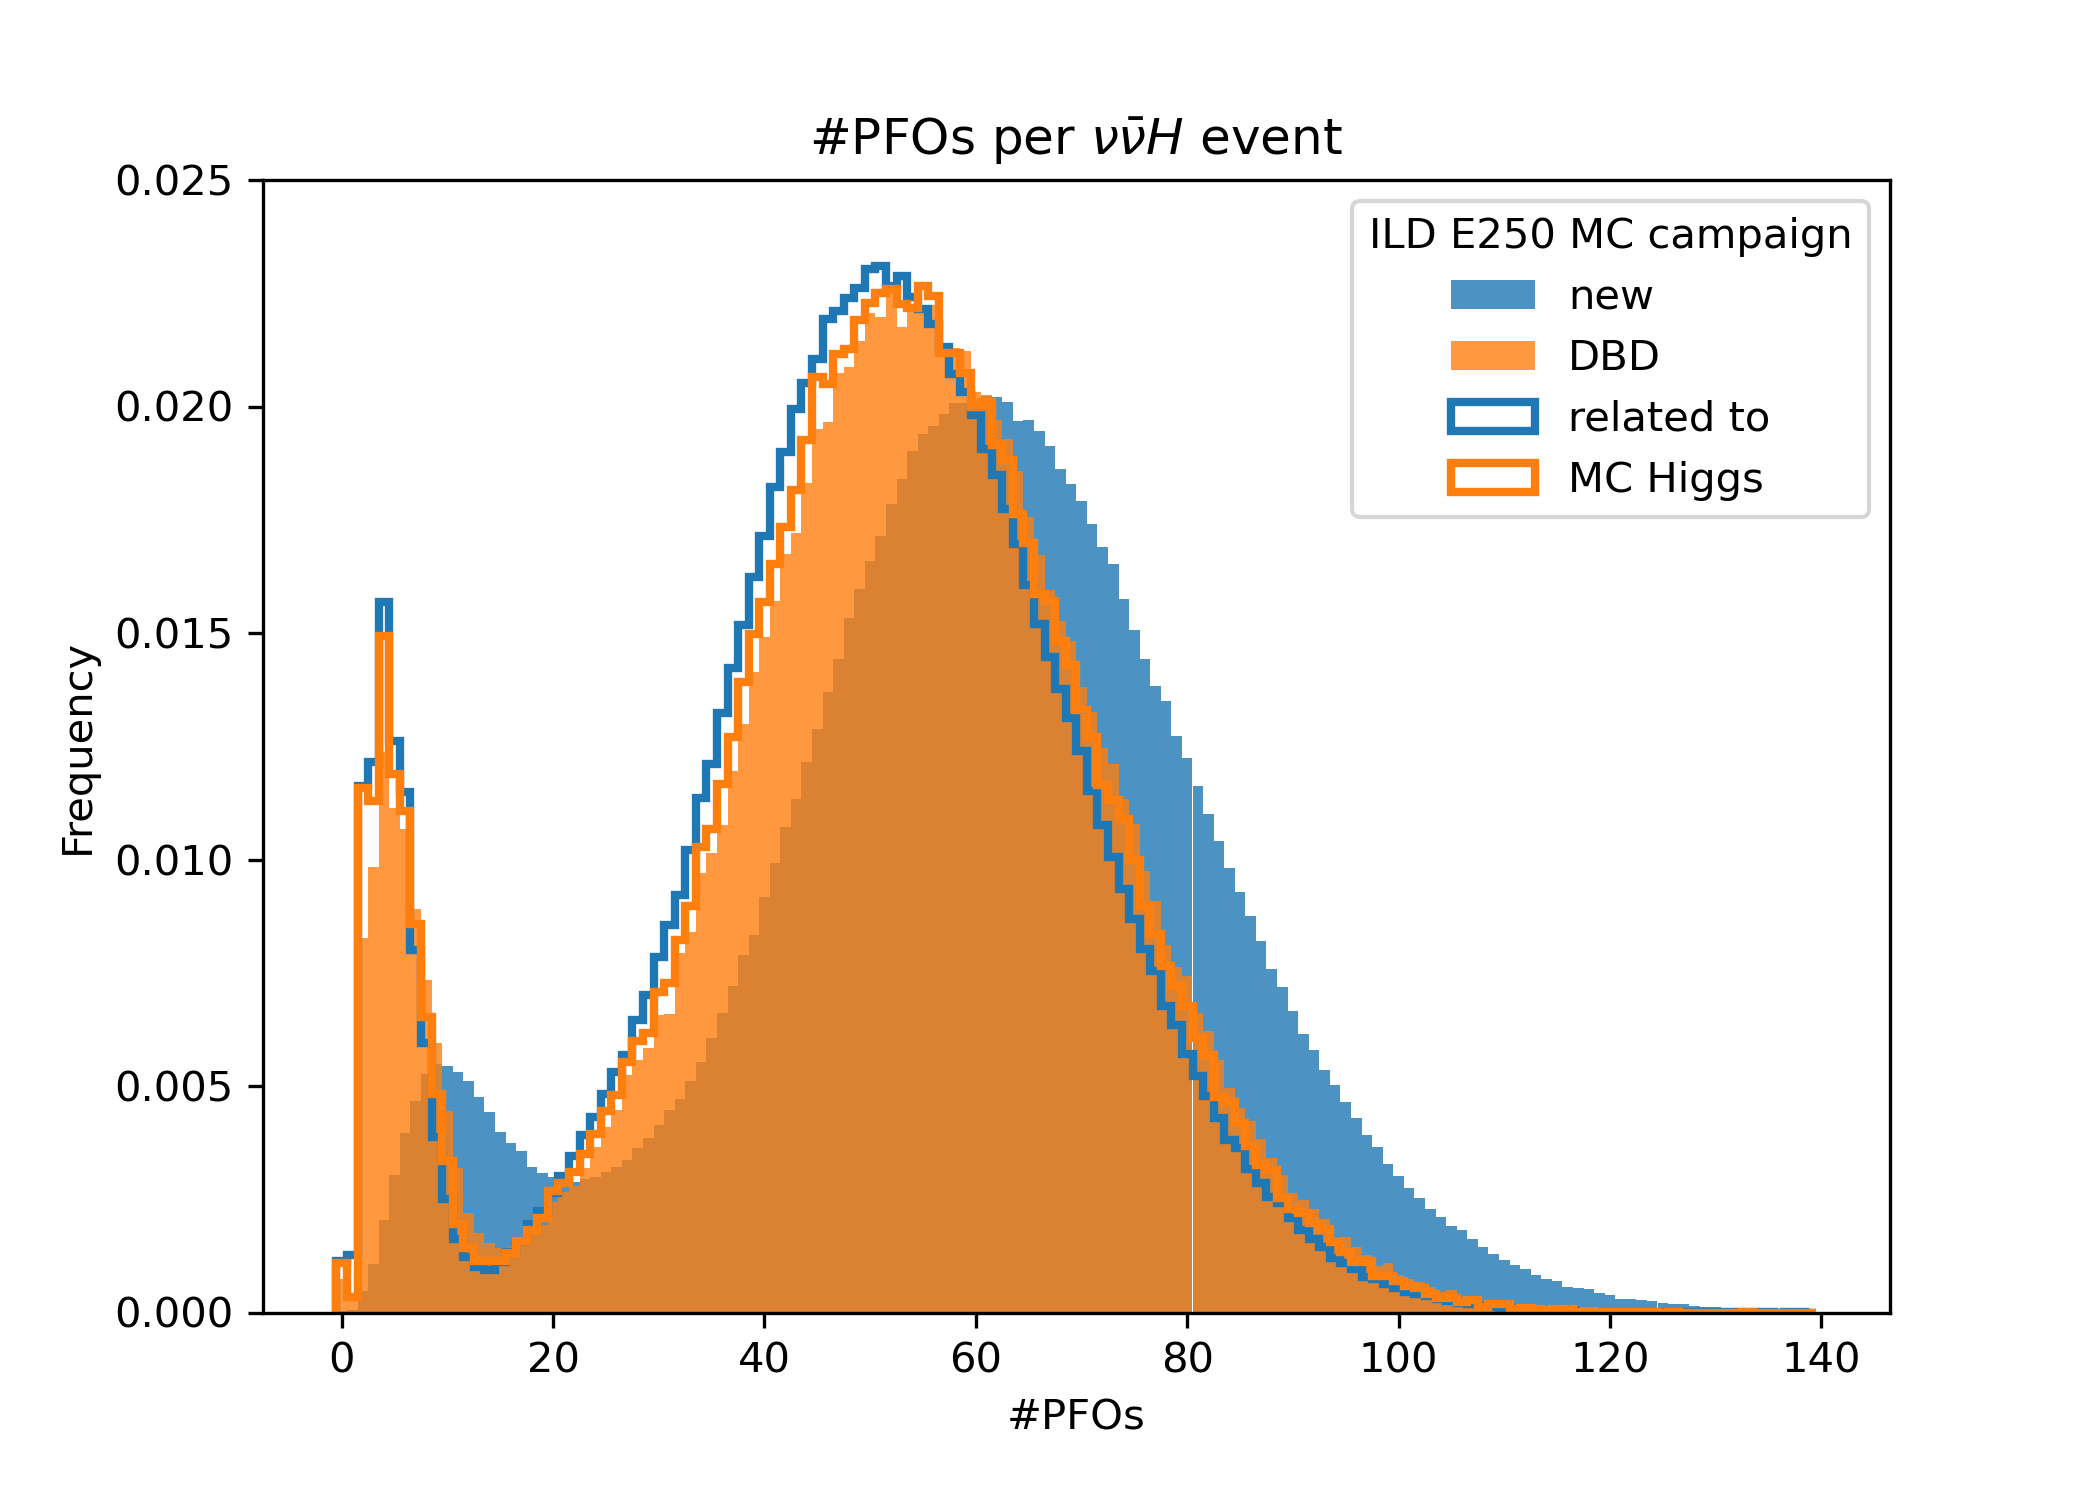
\includegraphics[height=\textheight, width=\textwidth, keepaspectratio]
        {n_pfos_full_and_only_higgs}}};
  \end{tikzpicture}
  \end{column}
  \end{columns}
  \end{frame}

\begin{frame}
  \frametitle{\textit{Global} variables}
  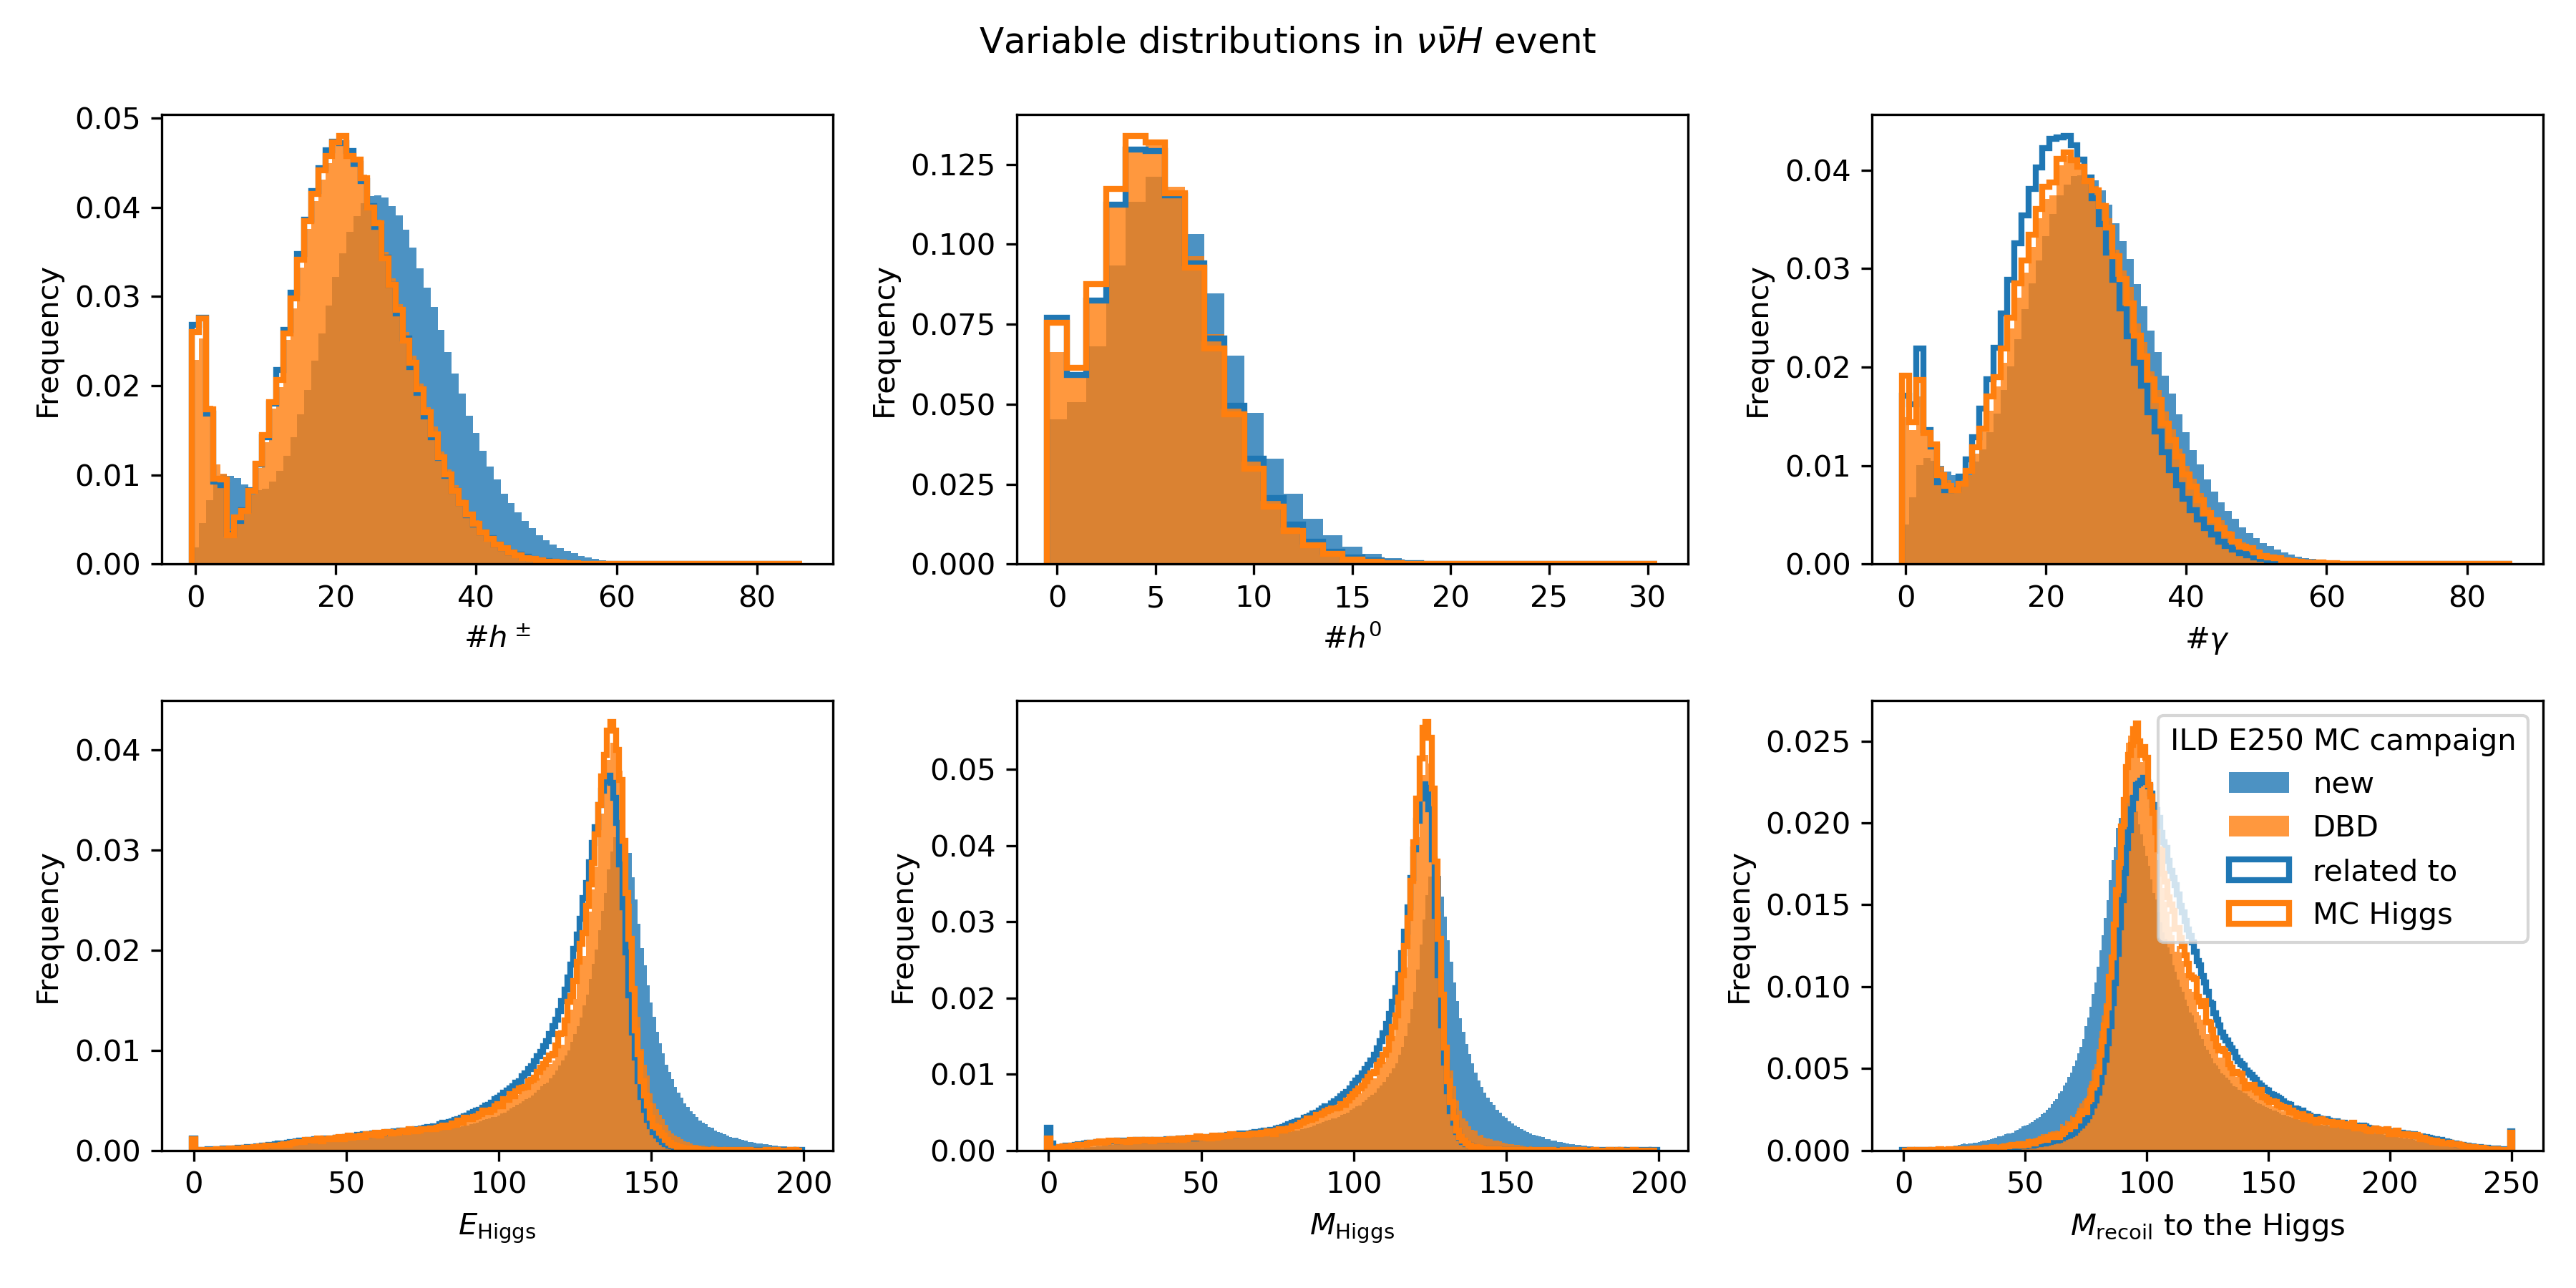
\includegraphics[height=0.9\textheight, width=\textwidth, keepaspectratio]
      {many_variables_full_and_only_higgs}
  \end{frame}

\begin{frame}
  \frametitle{Overlay composition}
  Frequency and size of the overlay increased, composition altered.
  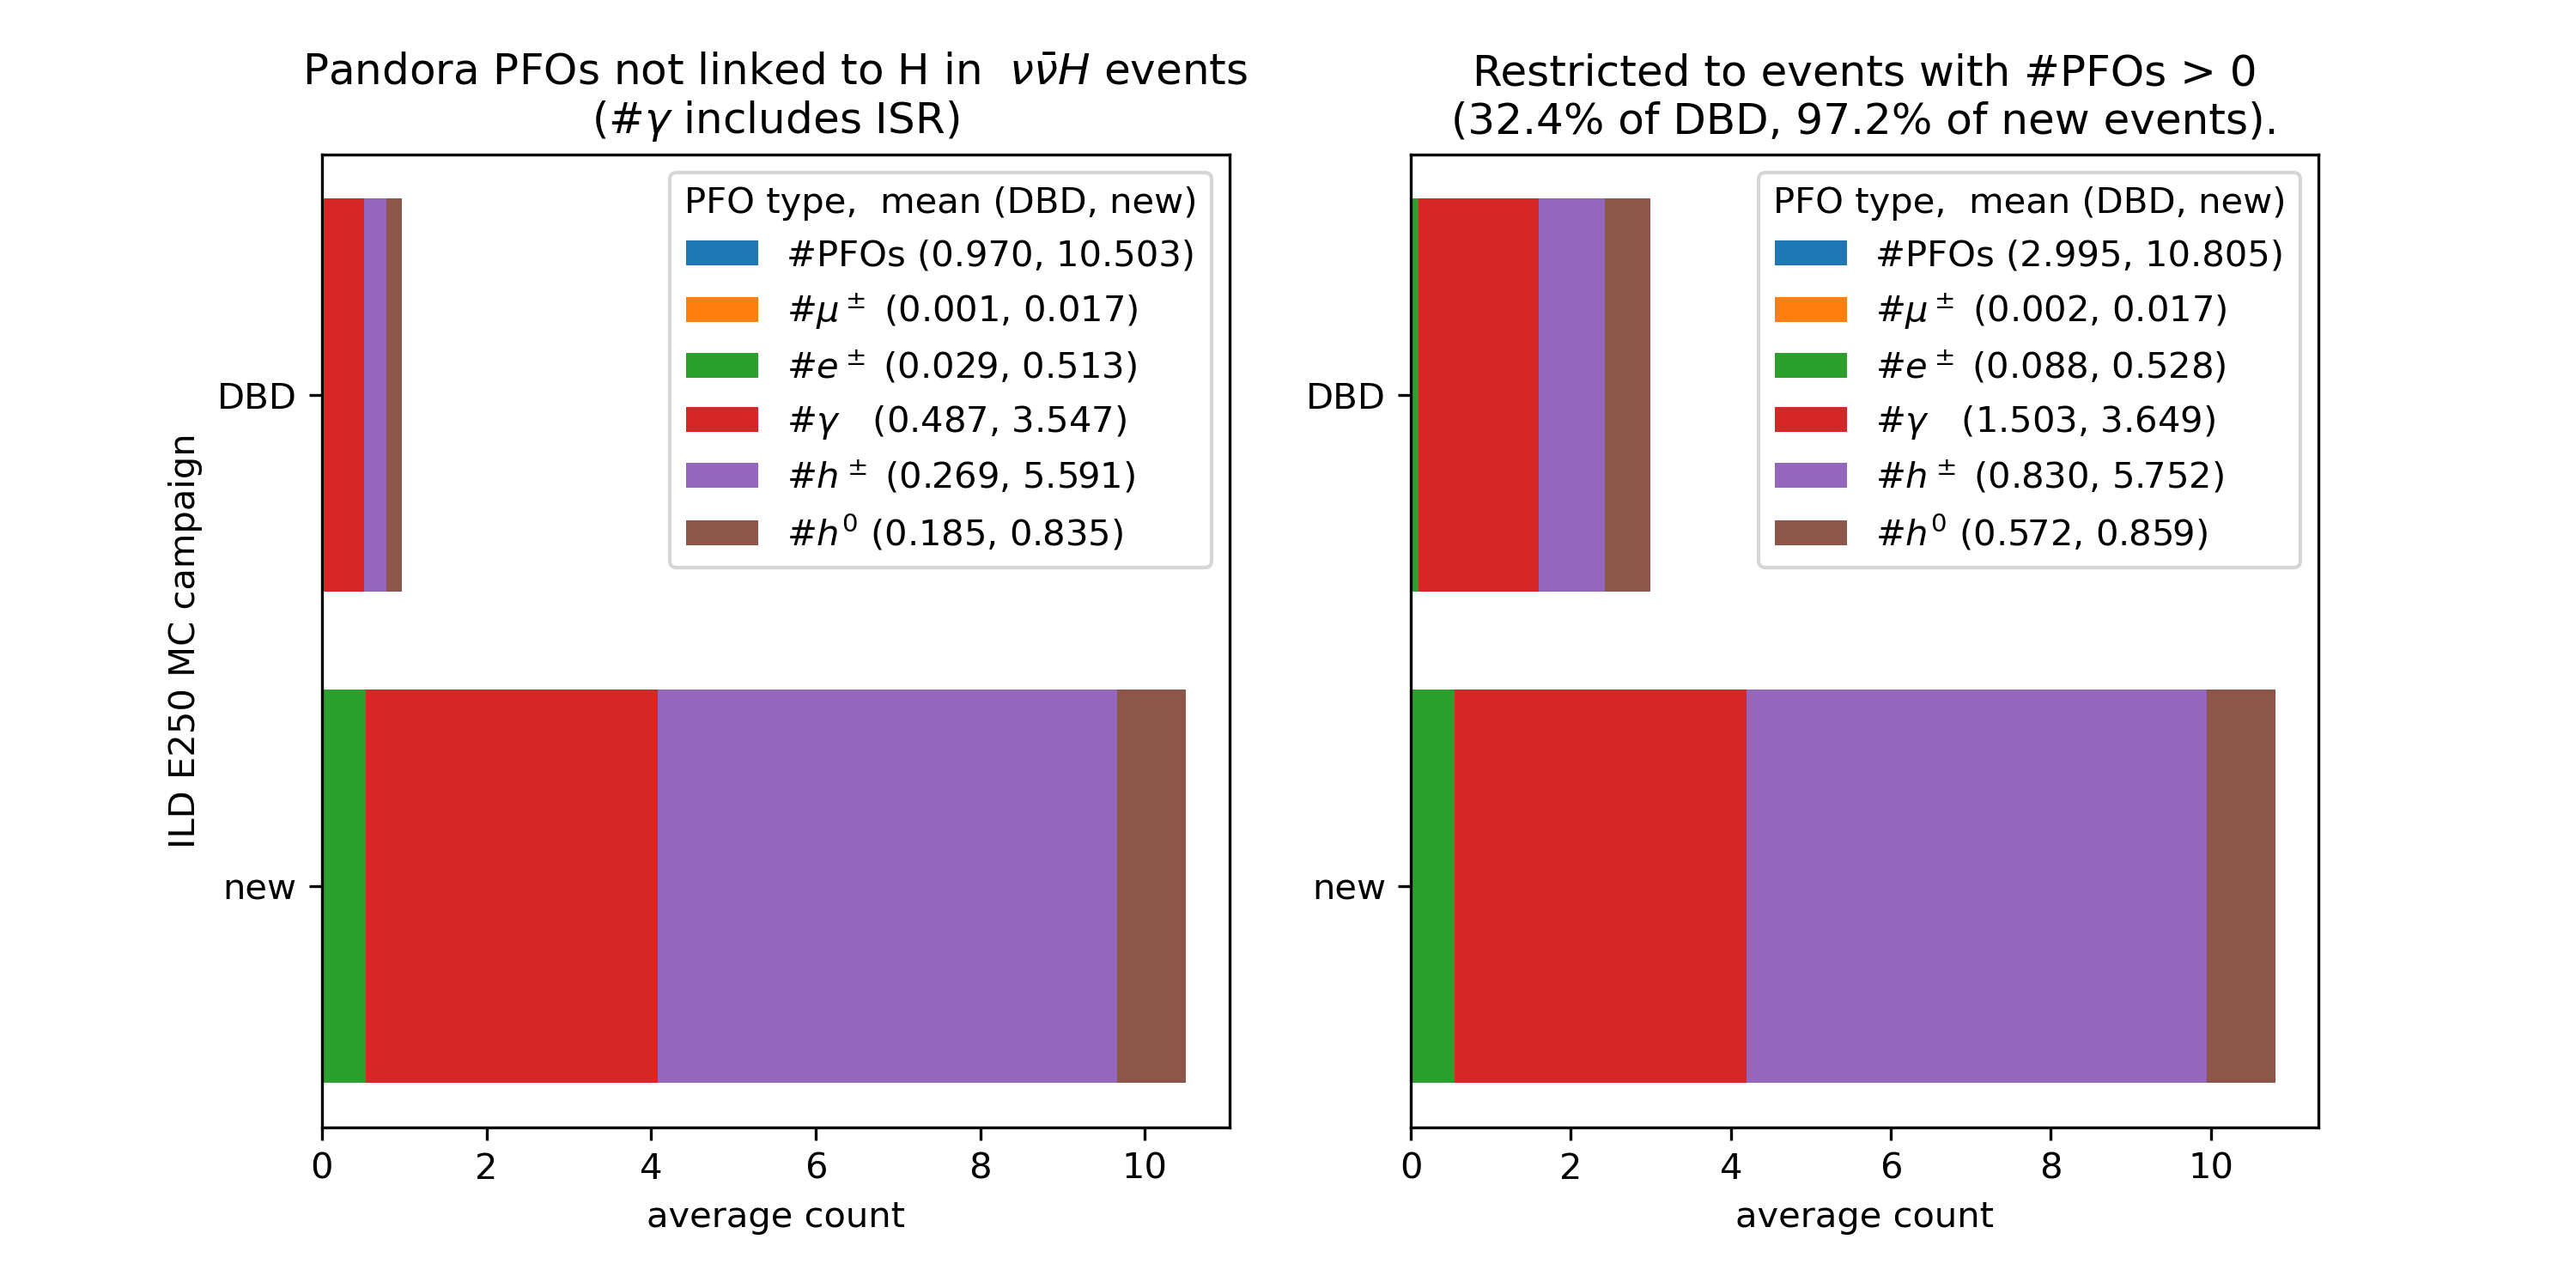
\includegraphics[height=0.8\textheight, width=\textwidth, keepaspectratio]
      {overlay_counts_per_group}
  \end{frame}

\begin{frame}
  \frametitle{Overlay shape}
  Frequency and size of the overlay increased, composition altered.
  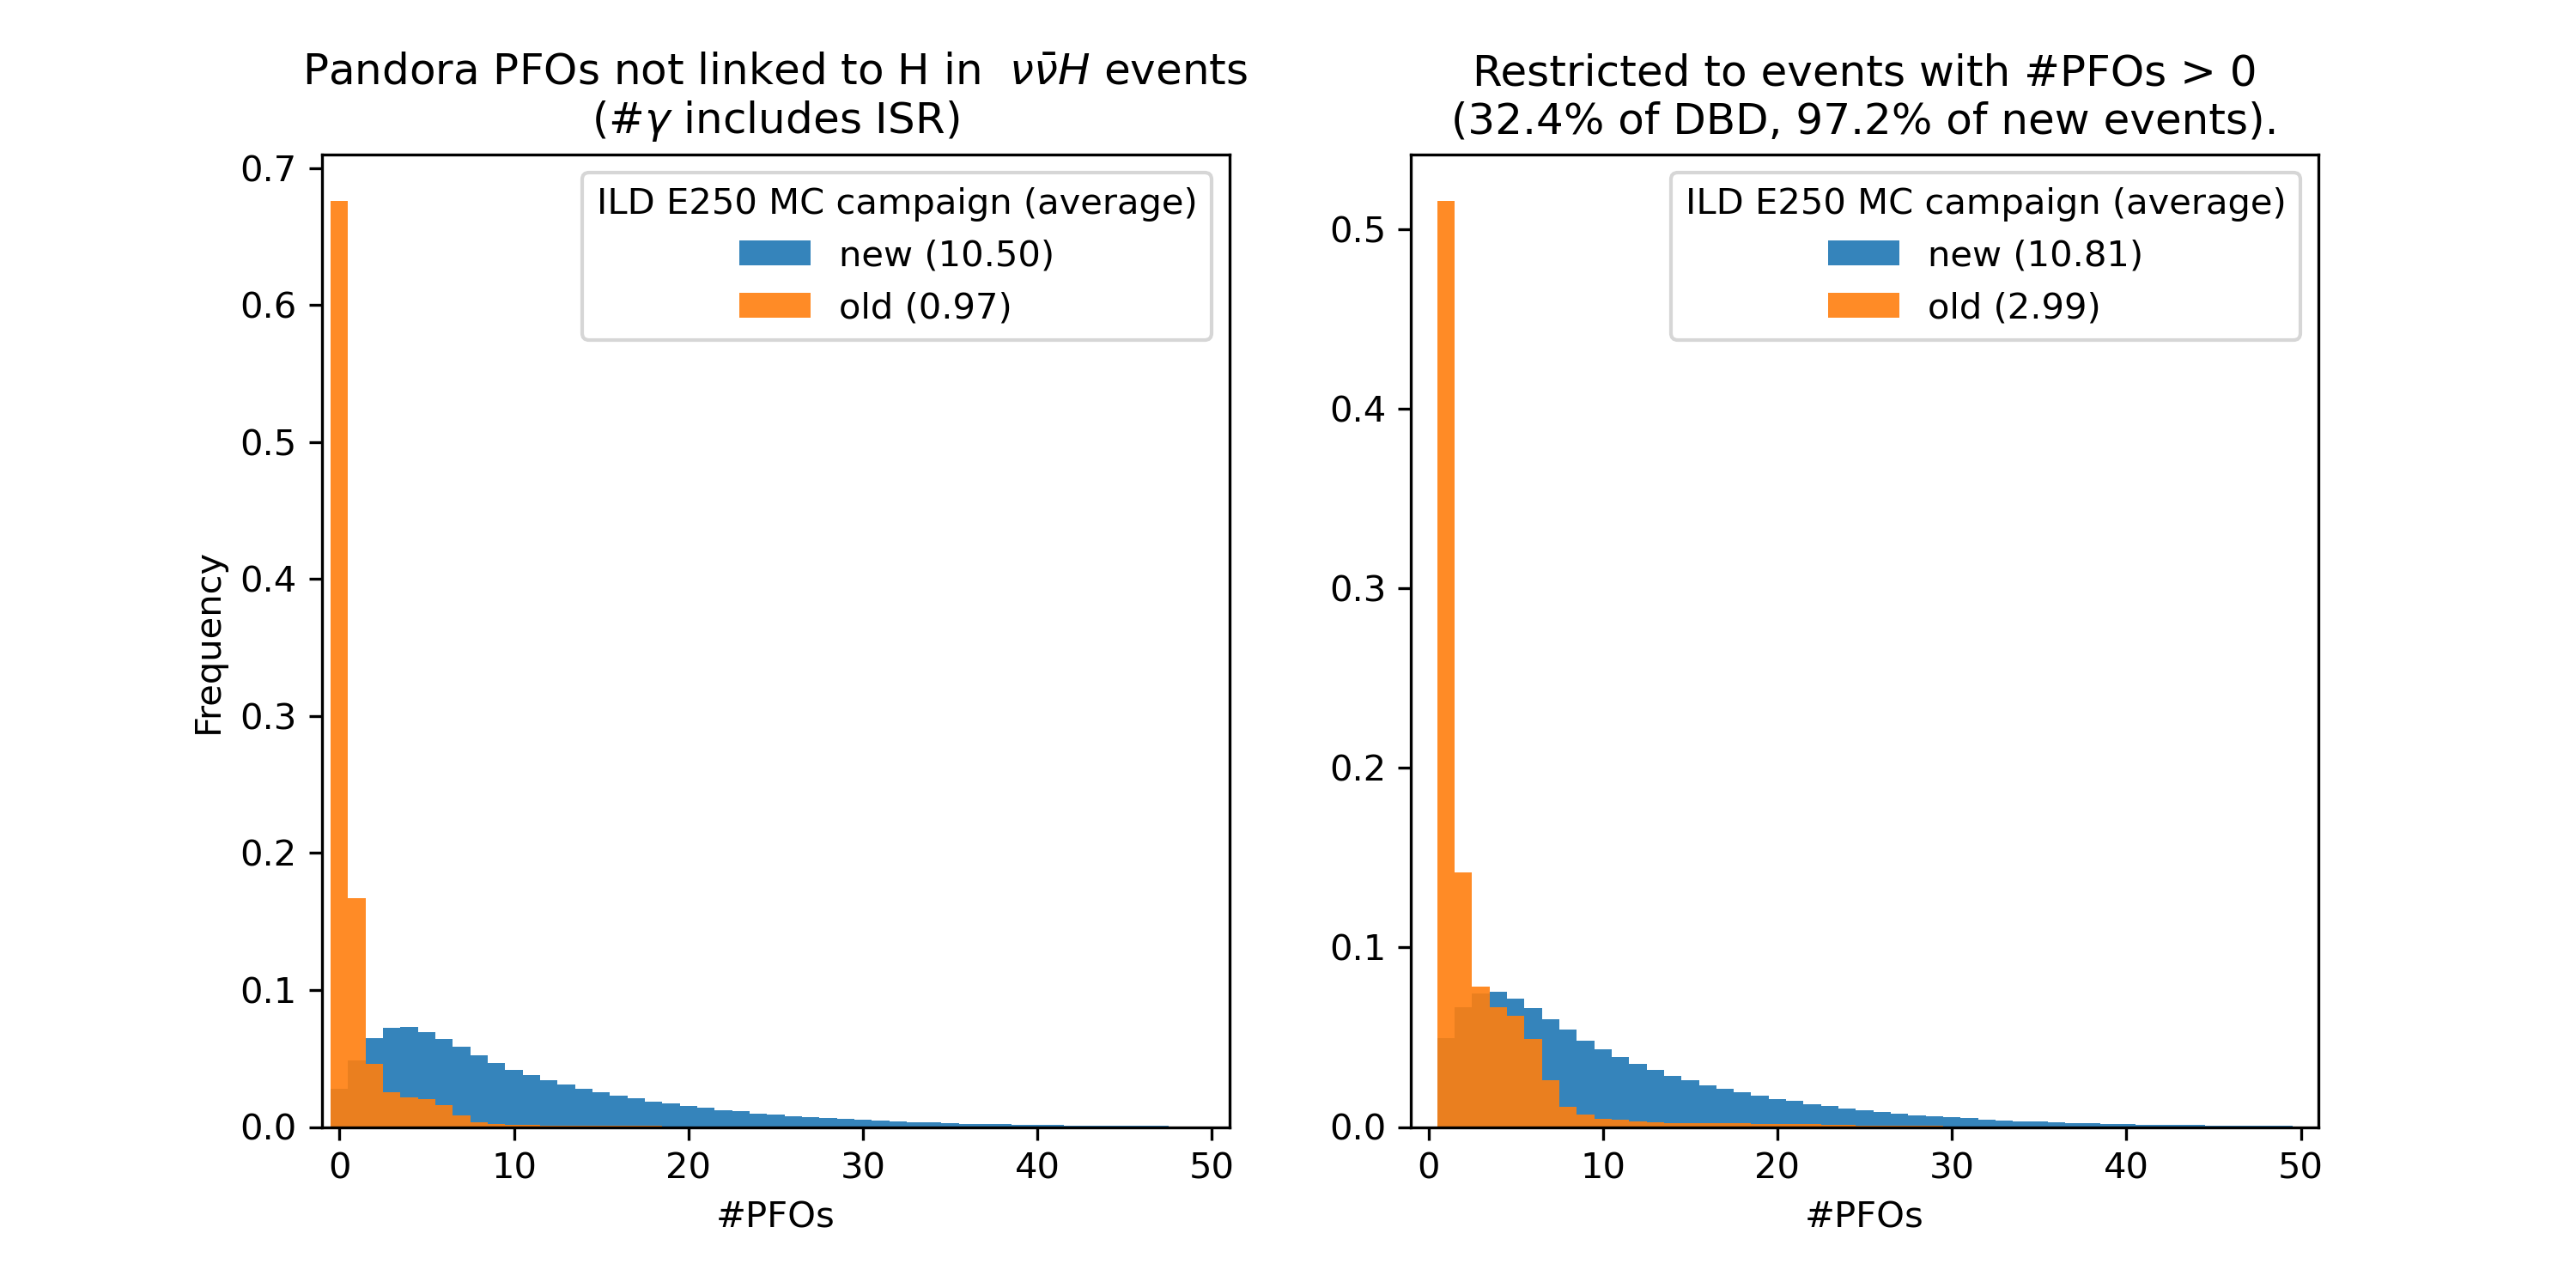
\includegraphics[height=0.8\textheight, width=\textwidth, keepaspectratio]
      {overlay_n_pfos}
  \end{frame}

\begin{frame}
  \frametitle{Overlay shape - log scale}
  Frequency and size of the overlay increased, composition altered.
  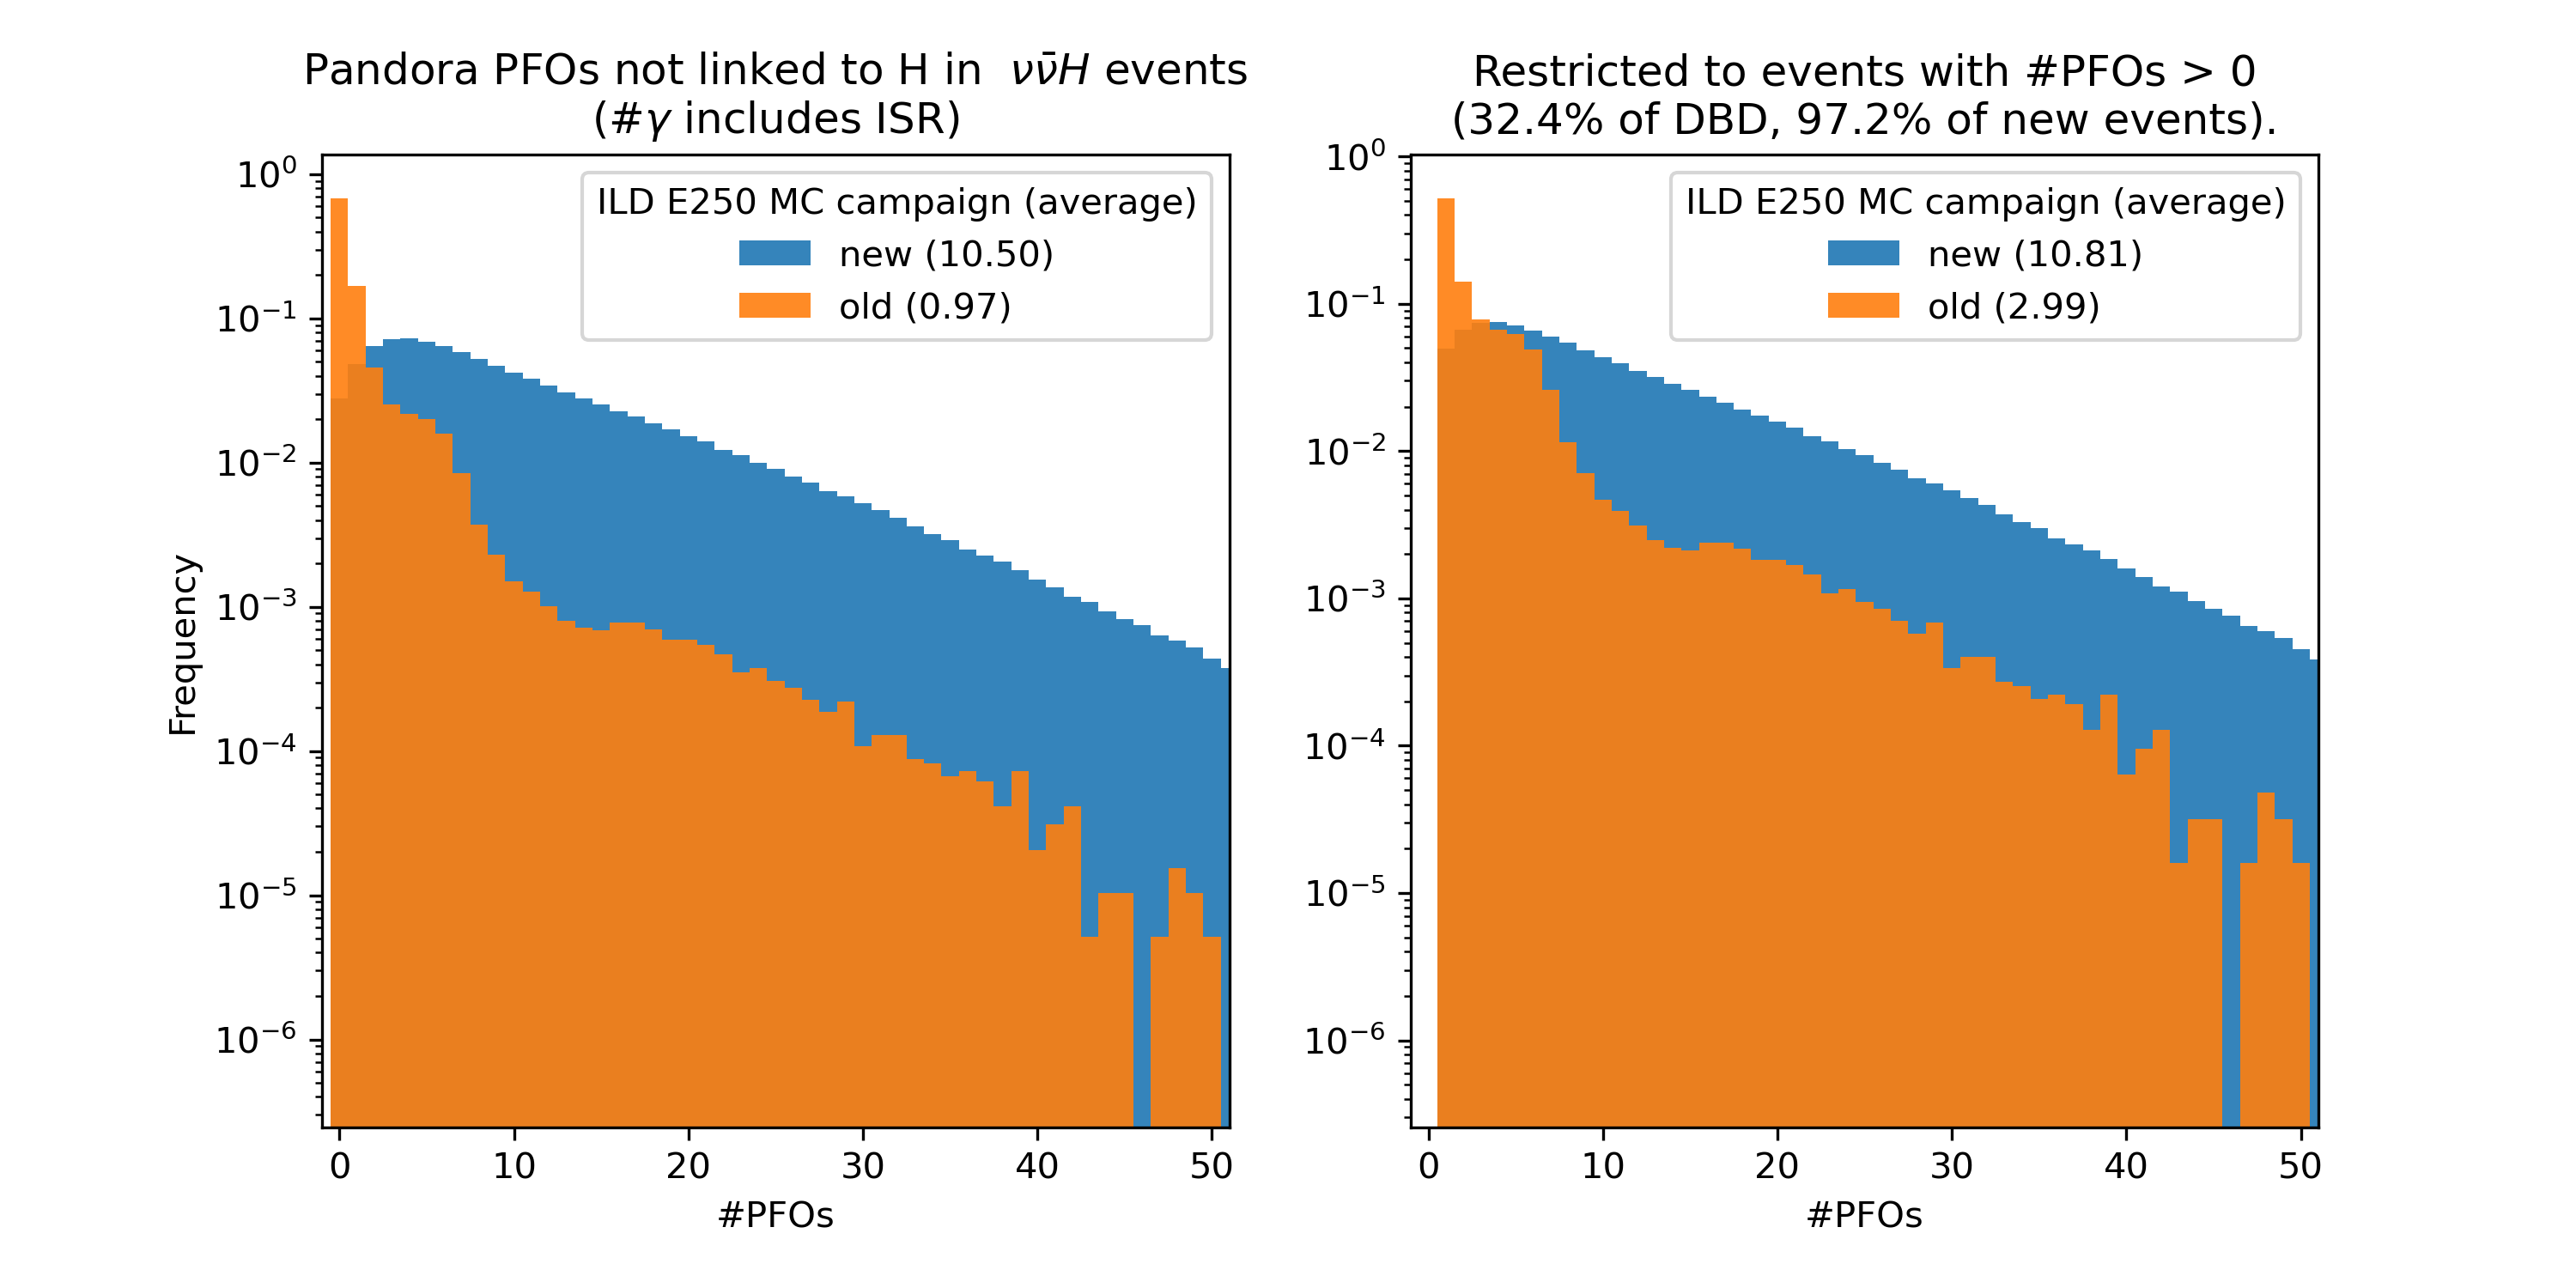
\includegraphics[height=0.8\textheight, width=\textwidth, keepaspectratio]
      {overlay_n_pfos_log}
  \end{frame}

\begin{frame}
  \frametitle{Overlay energy}
  On average $\approx10~\GeV$. $E_{\tn{Higgs}}^{\tn{mean}}\approx130~\GeV$.
  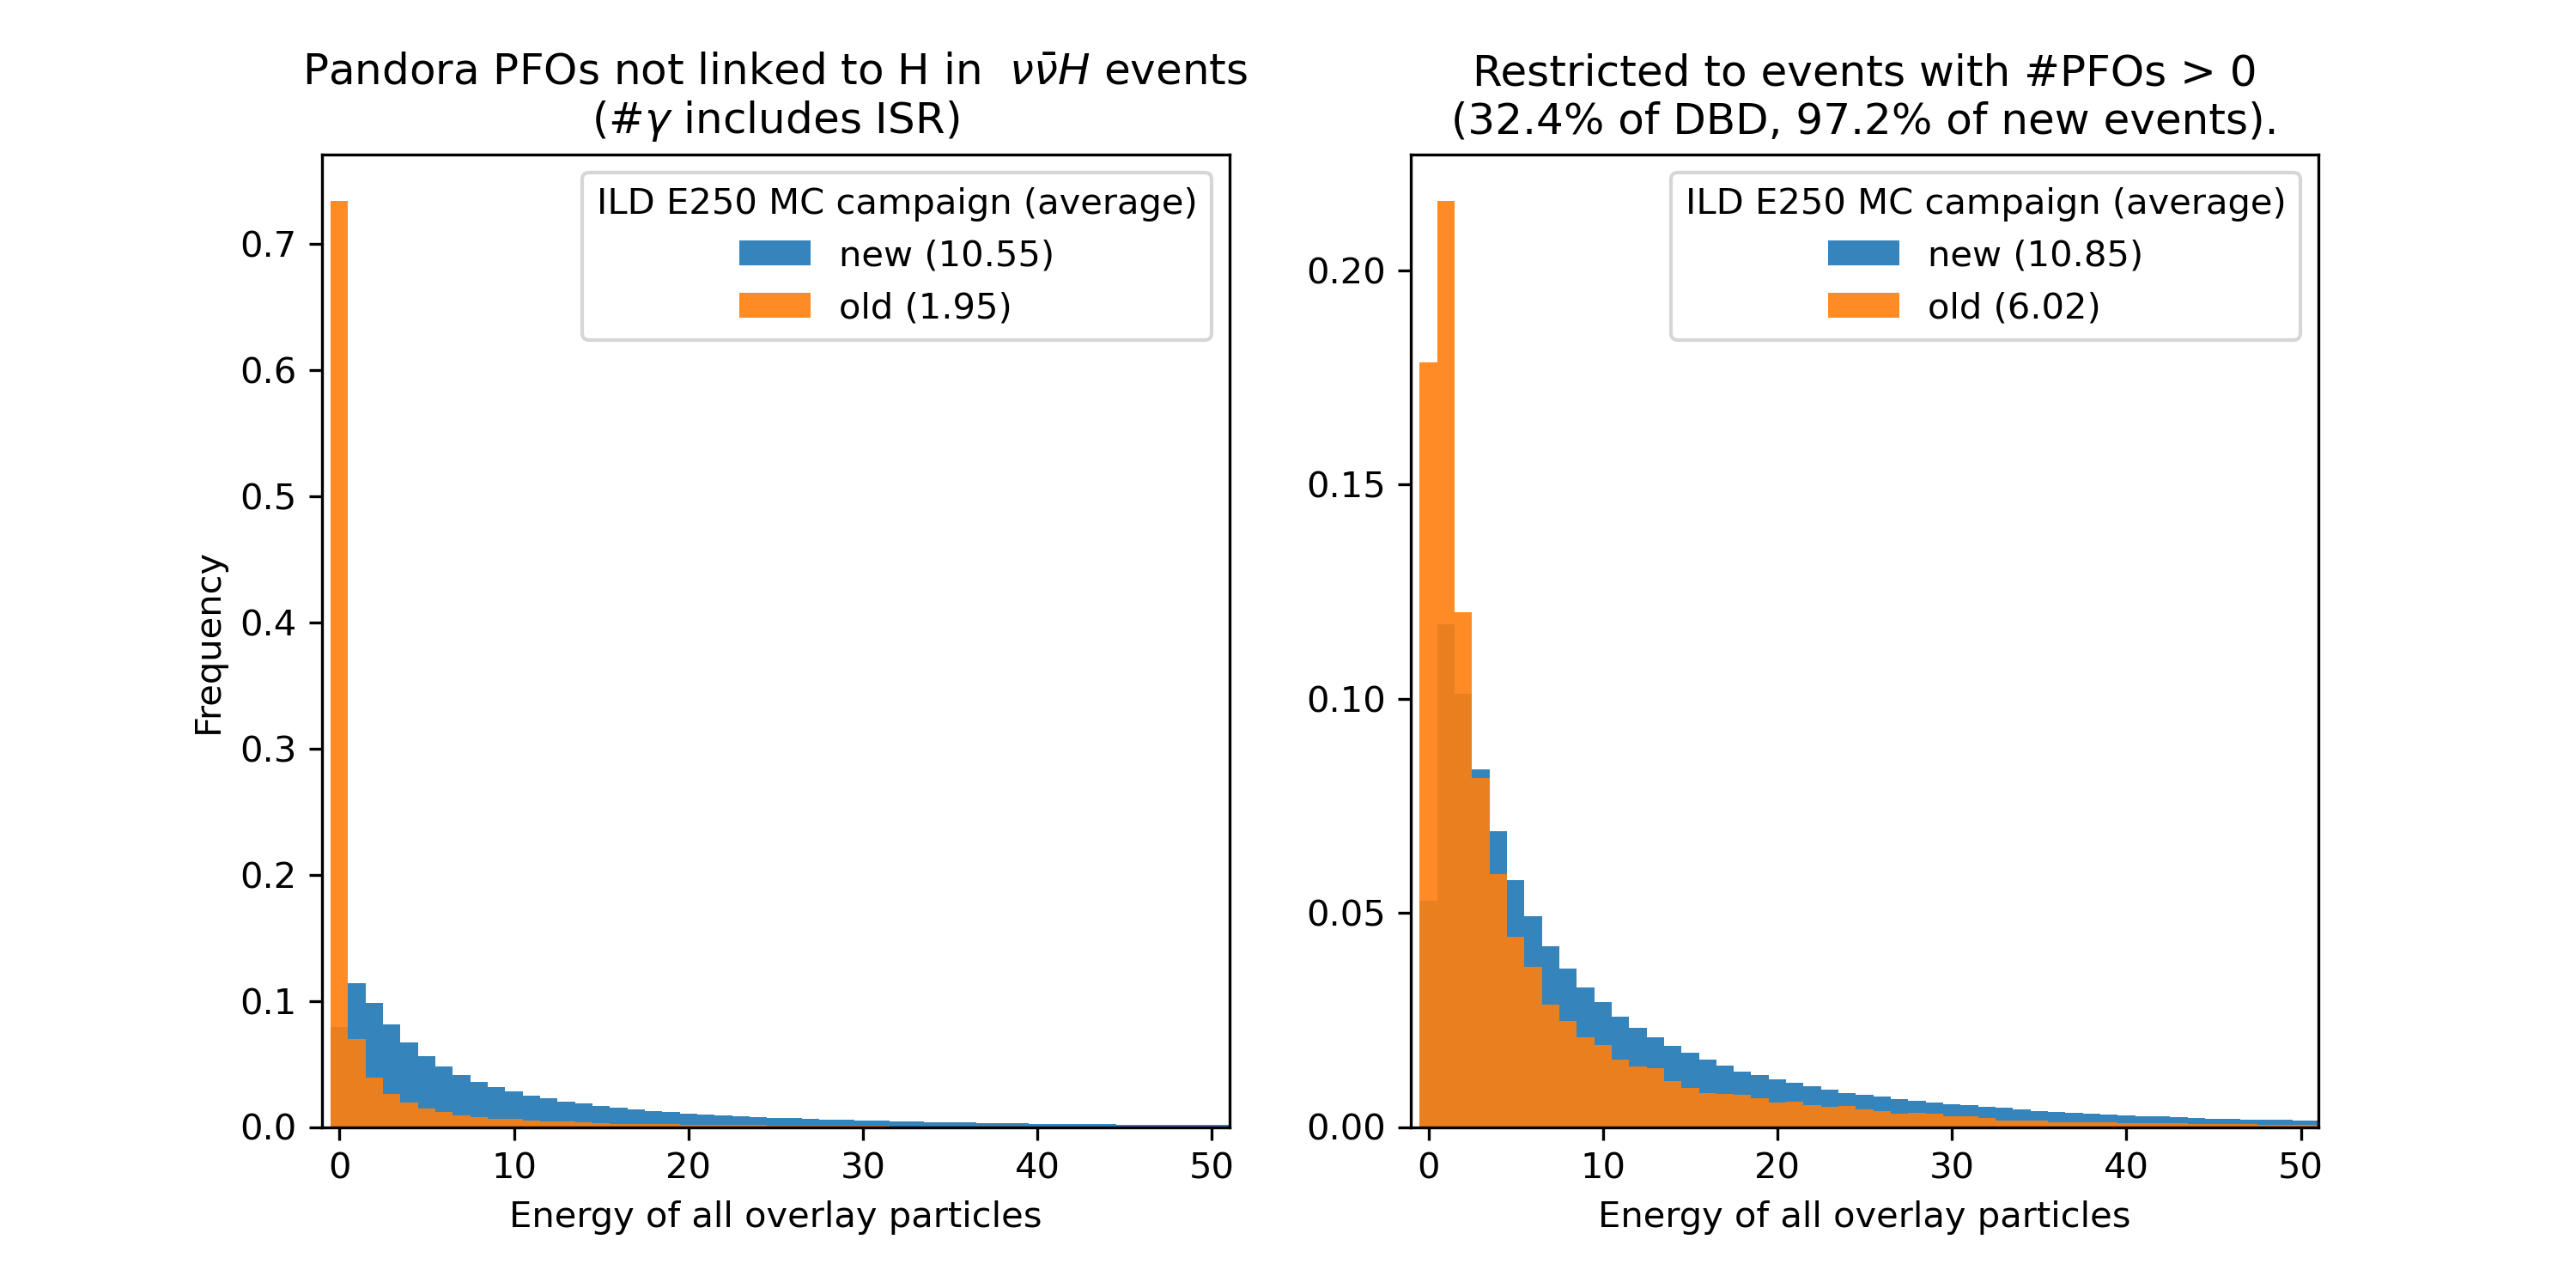
\includegraphics[height=0.8\textheight, width=\textwidth, keepaspectratio]
      {overlay_energy}
  \end{frame}

\begin{frame}
  \frametitle{Overlay energy}
  On average $\approx10~\GeV$. $E_{\tn{Higgs}}^{\tn{mean}}\approx130~\GeV$.
  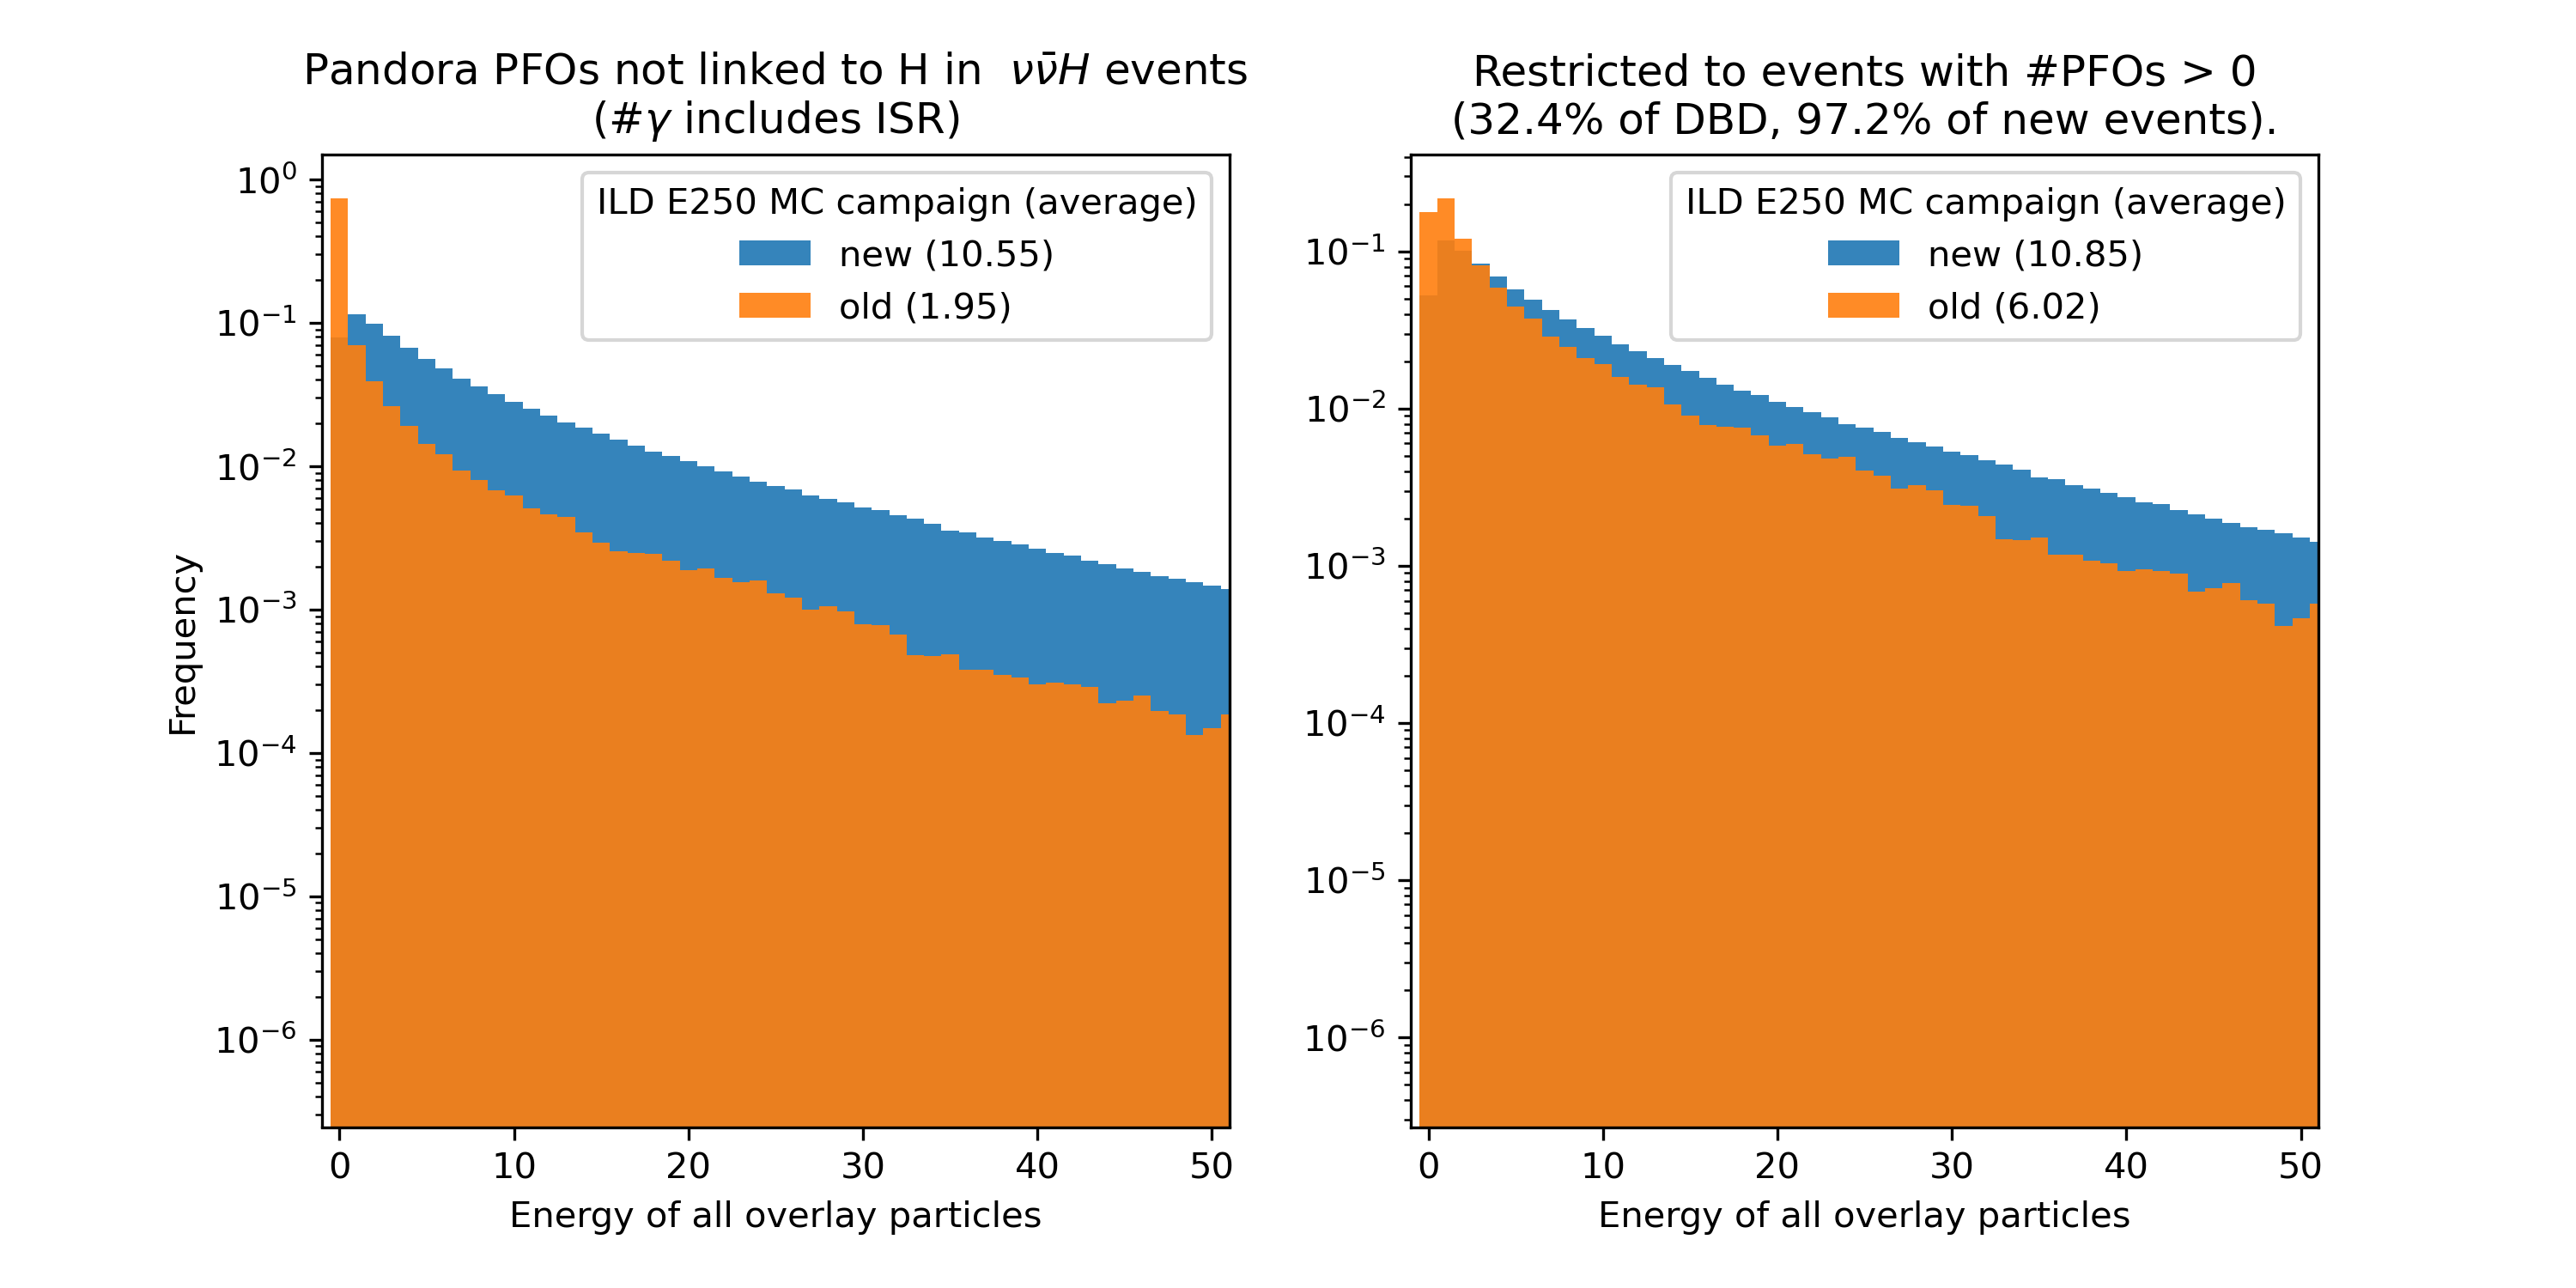
\includegraphics[height=0.8\textheight, width=\textwidth, keepaspectratio]
      {overlay_energy_log}
  \end{frame}

\begin{frame}
  \frametitle{Isolated Leptons}
  Using the IsolatedLeptonTaggingProcessor with DBD weights.
  \begin{center}
    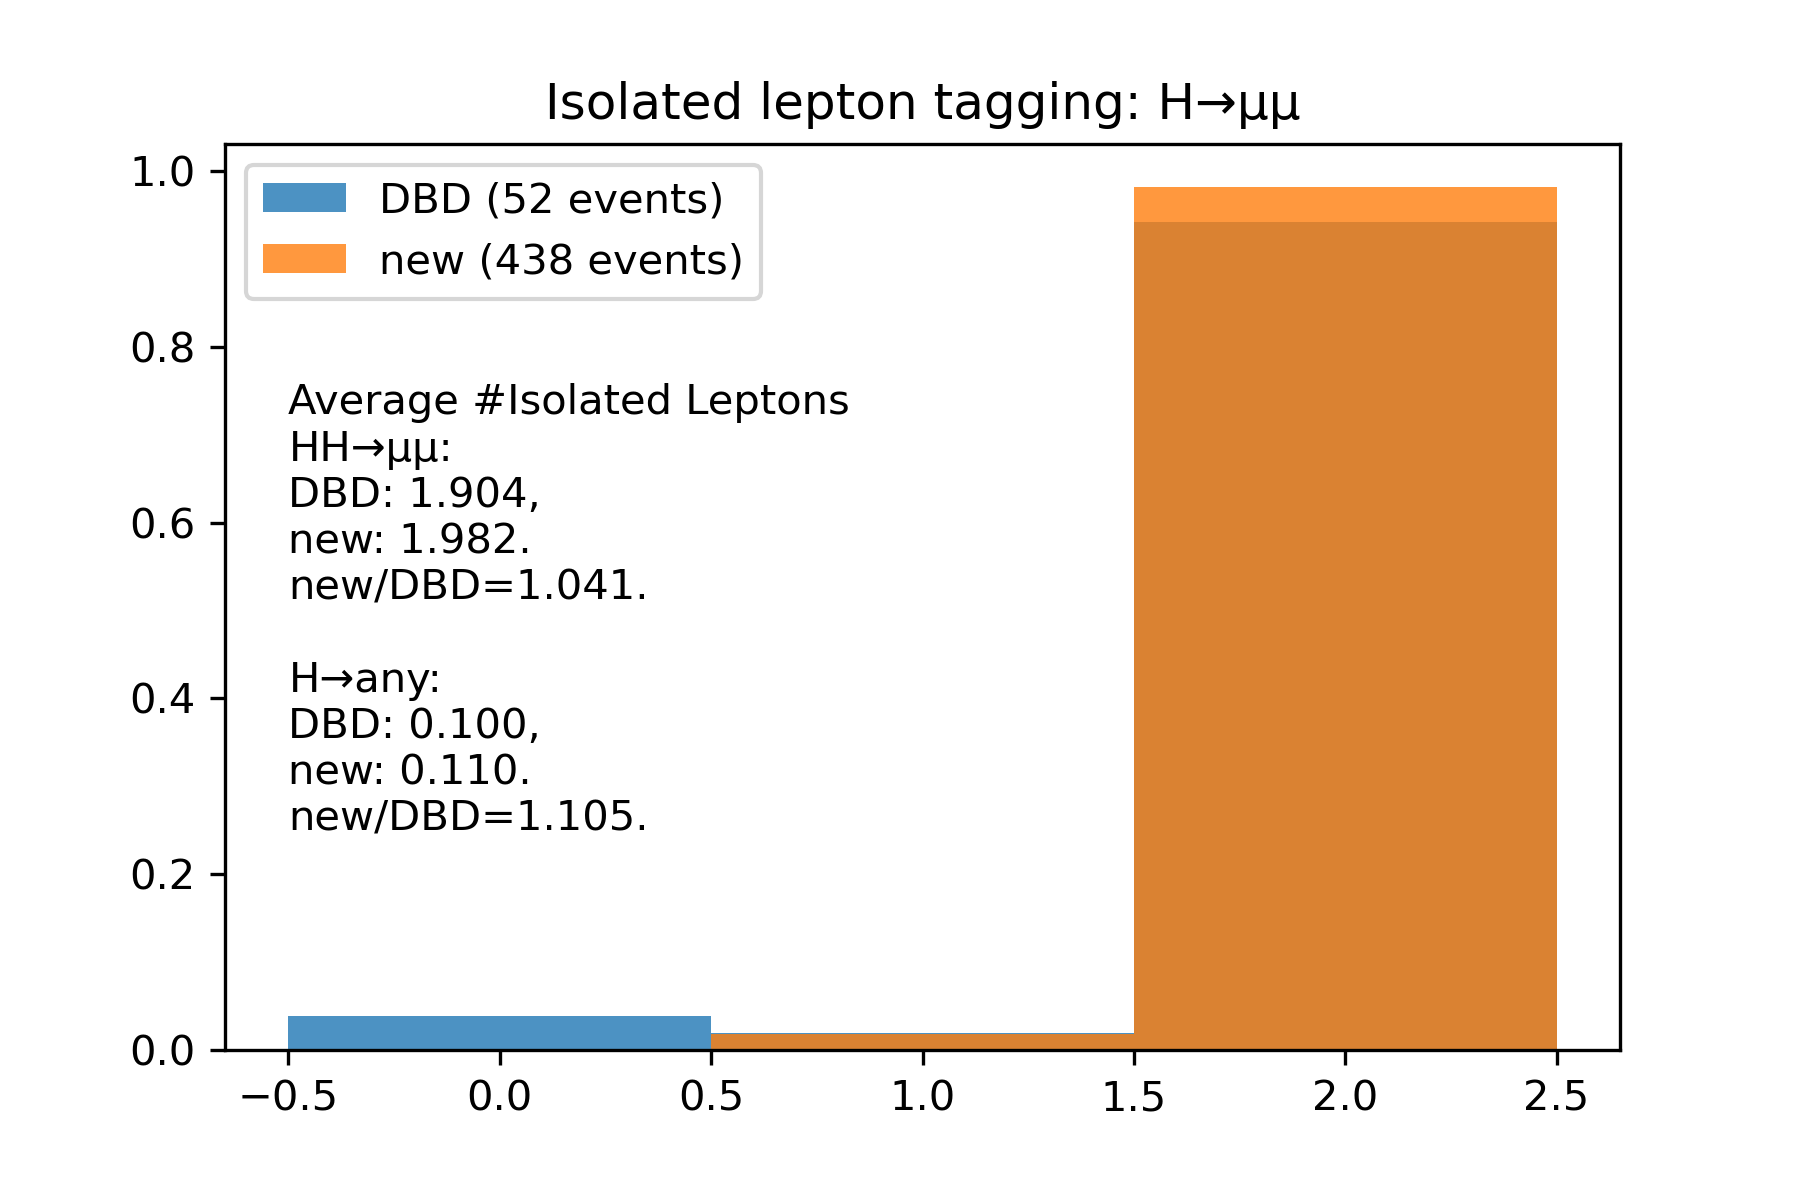
\includegraphics[height=0.8\textheight, width=\textwidth, keepaspectratio]
        {isolated_leptons}
  \end{center}
  \end{frame}

\begin{frame}
  \frametitle{Branching ratios}
  \begin{columns}[c,onlytextwidth]
  \begin{column}{0.5\textwidth}
  Differences (red) seem to be larger than statistical uncertainty.
  \newline\newline
  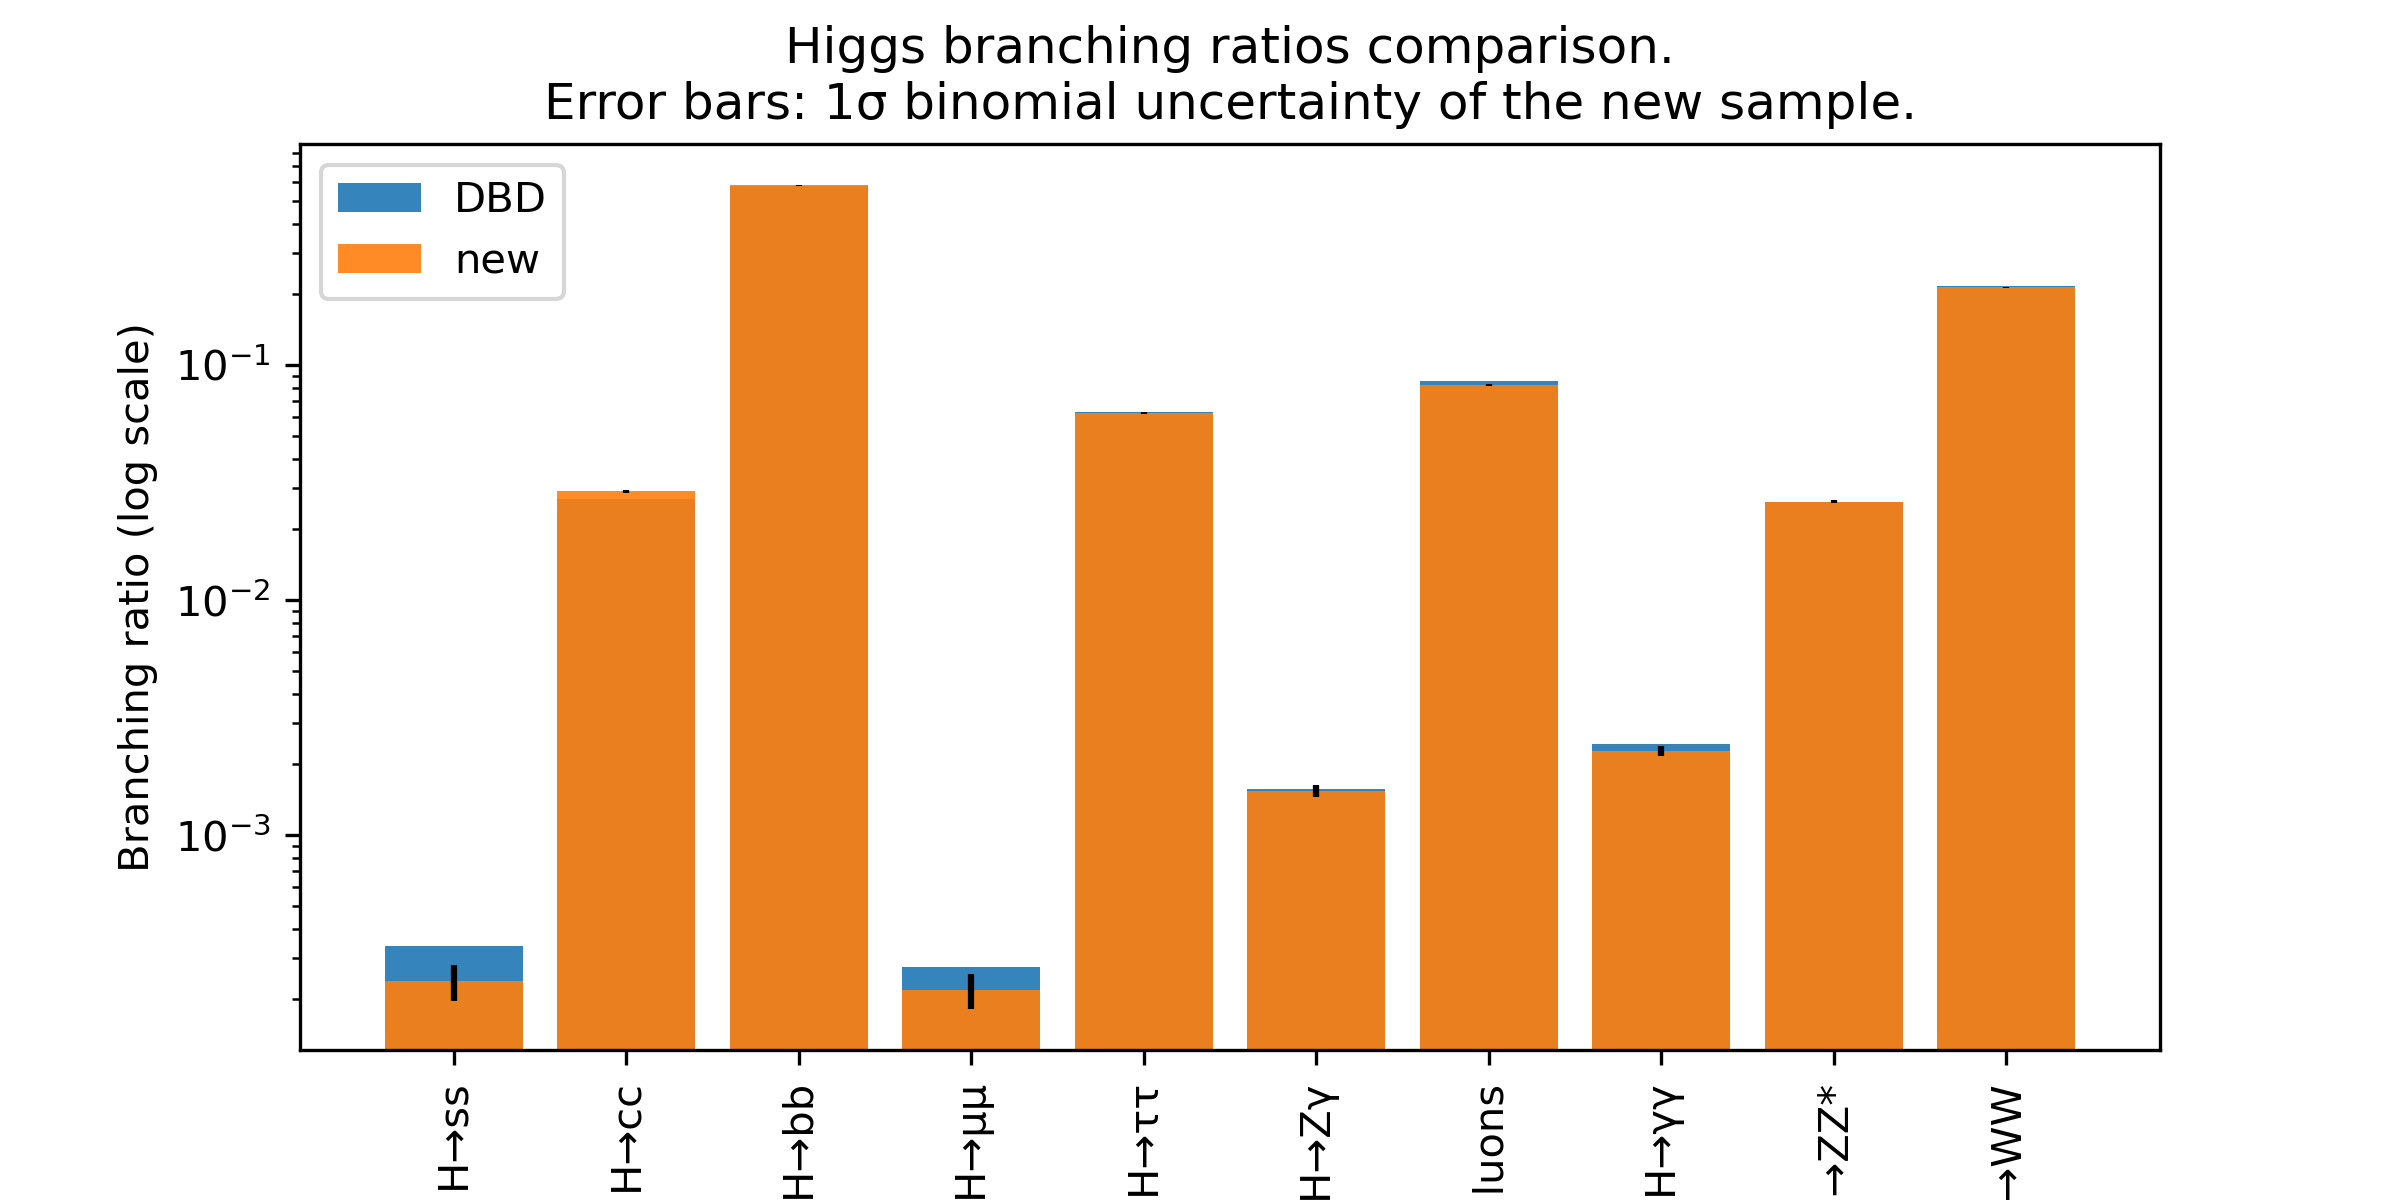
\includegraphics[width=.8\textwidth, keepaspectratio]
    {branching_ratio_difference_log}
  \end{column}
  \begin{column}{0.5\textwidth}
  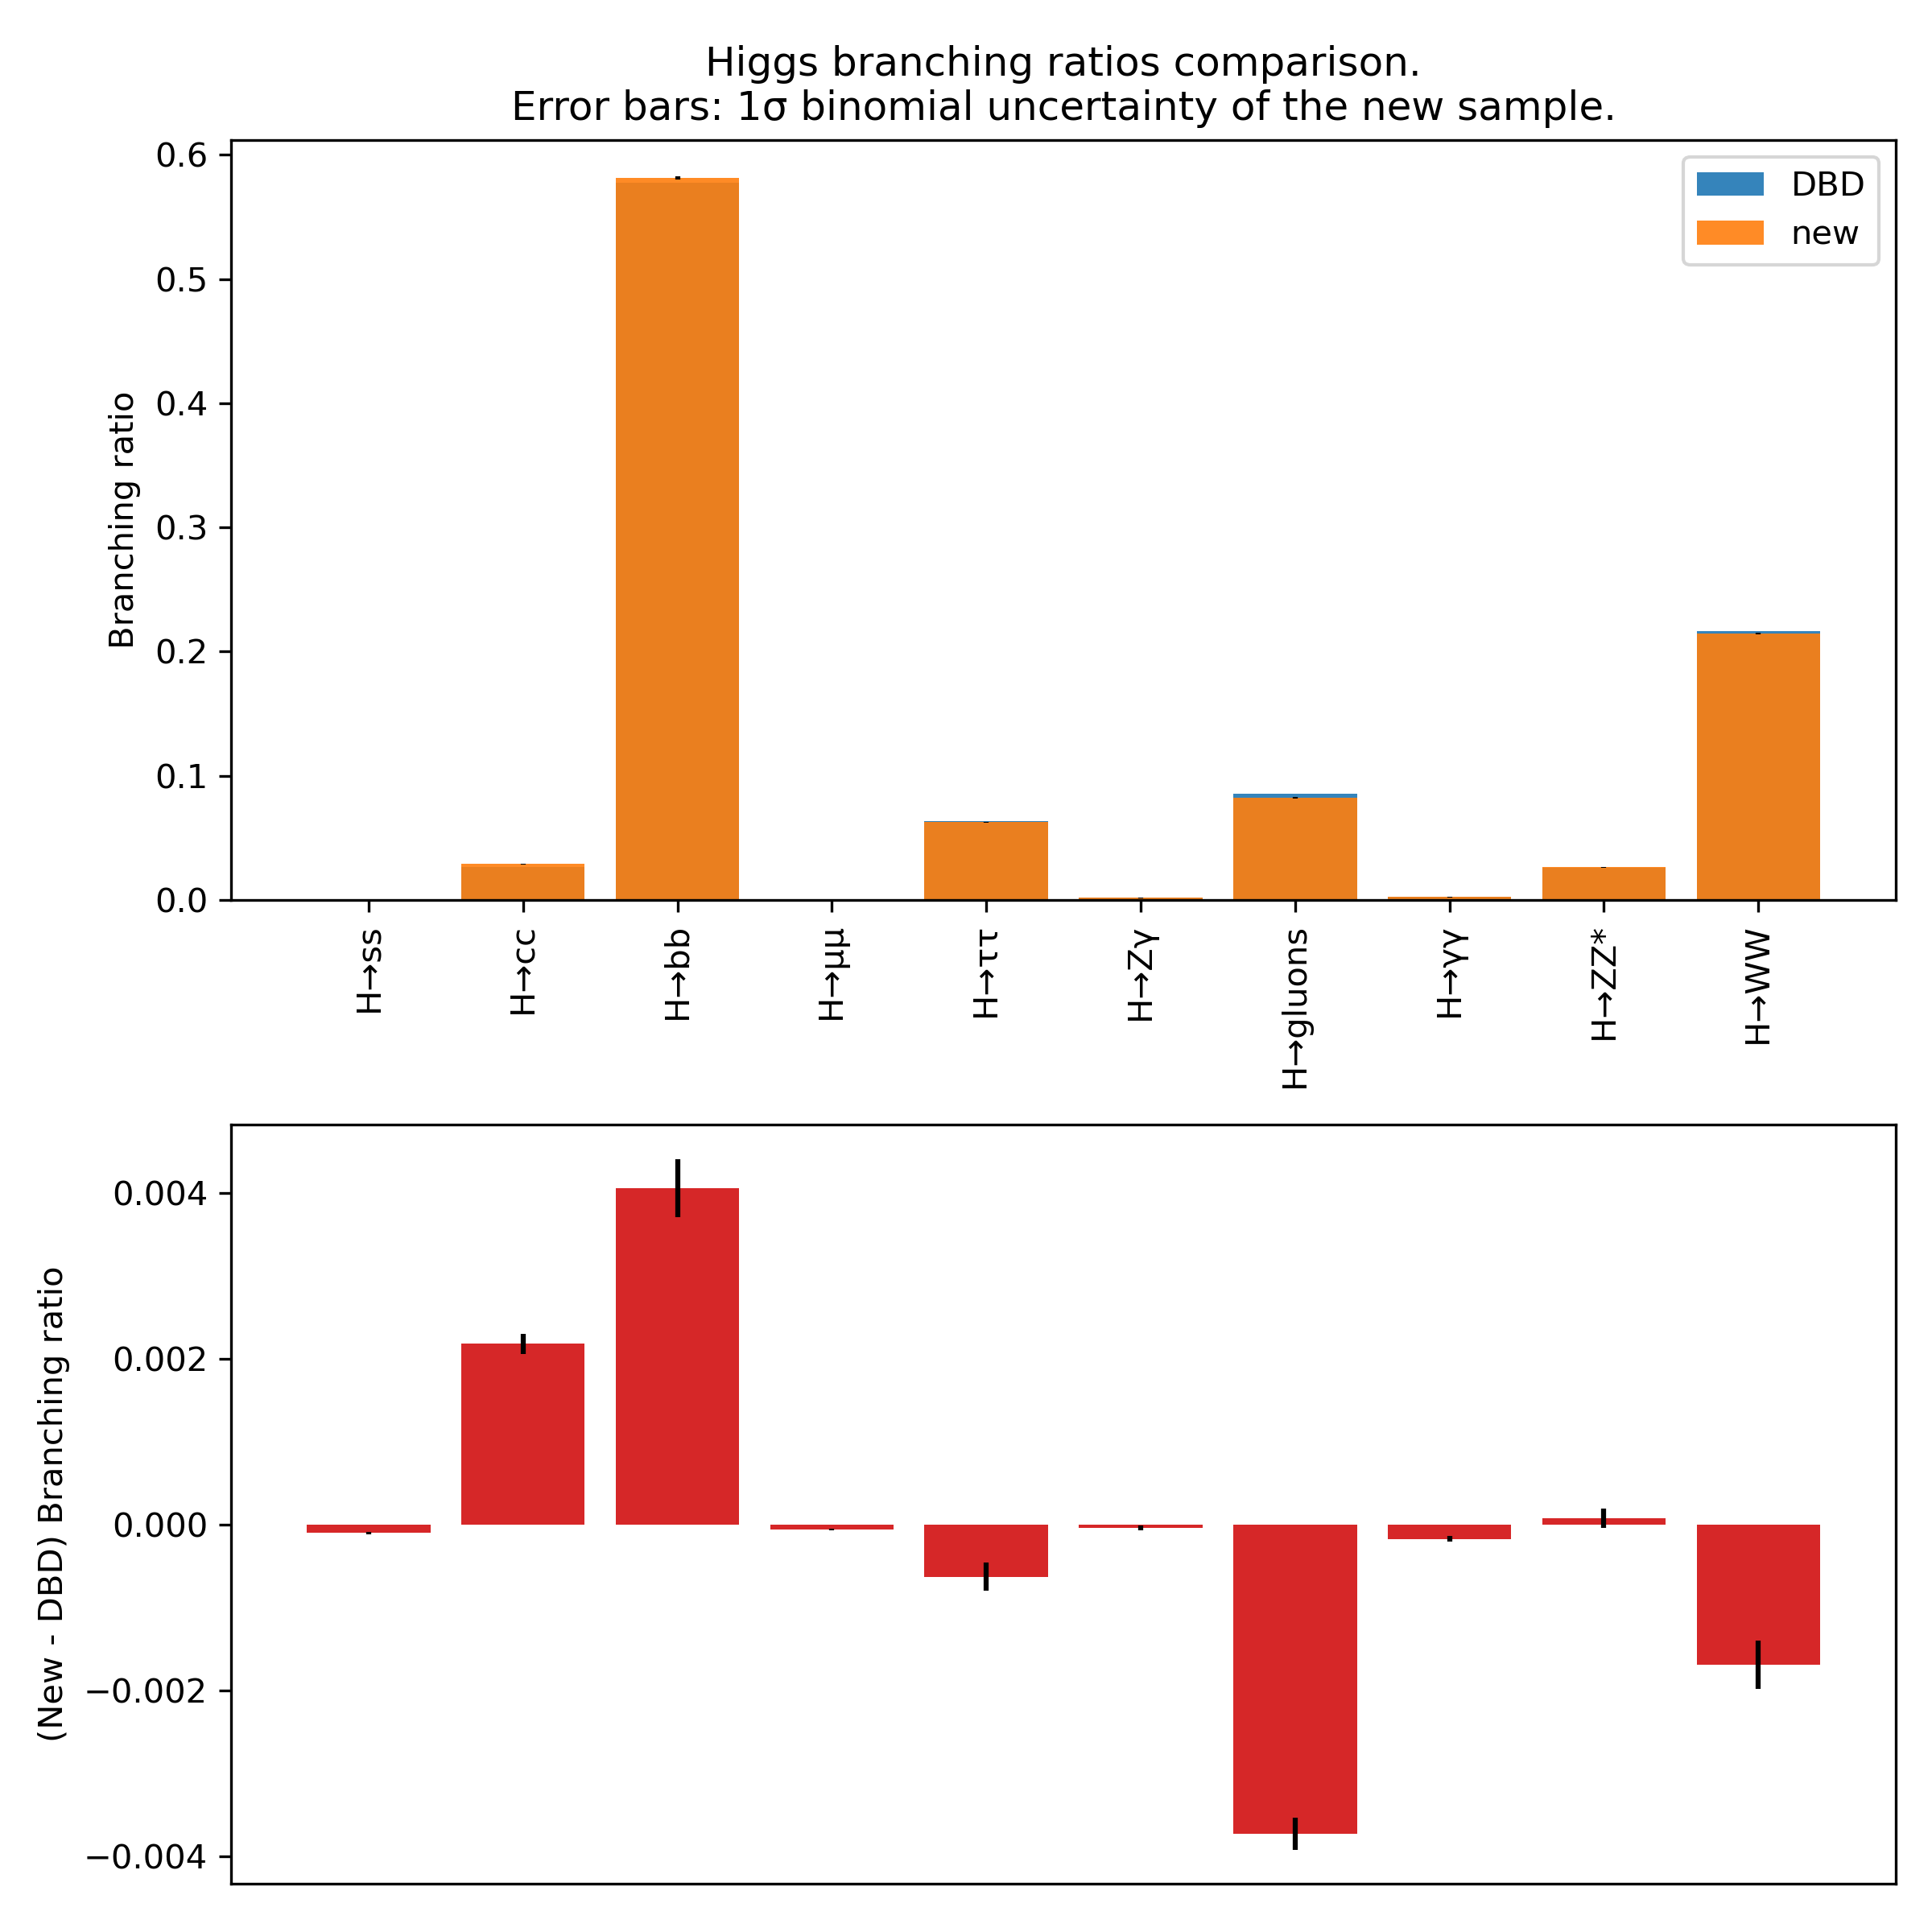
\includegraphics[width=.8\textwidth, keepaspectratio]
    {branching_ratio_difference}
  \end{column}
  \end{columns}
  \end{frame}

\begin{frame}
  \frametitle{\#PFOs per Higgs decay mode}
  Increased overlay makes it harder to use \textit{global} information.
  \begin{center}
  \only<1>{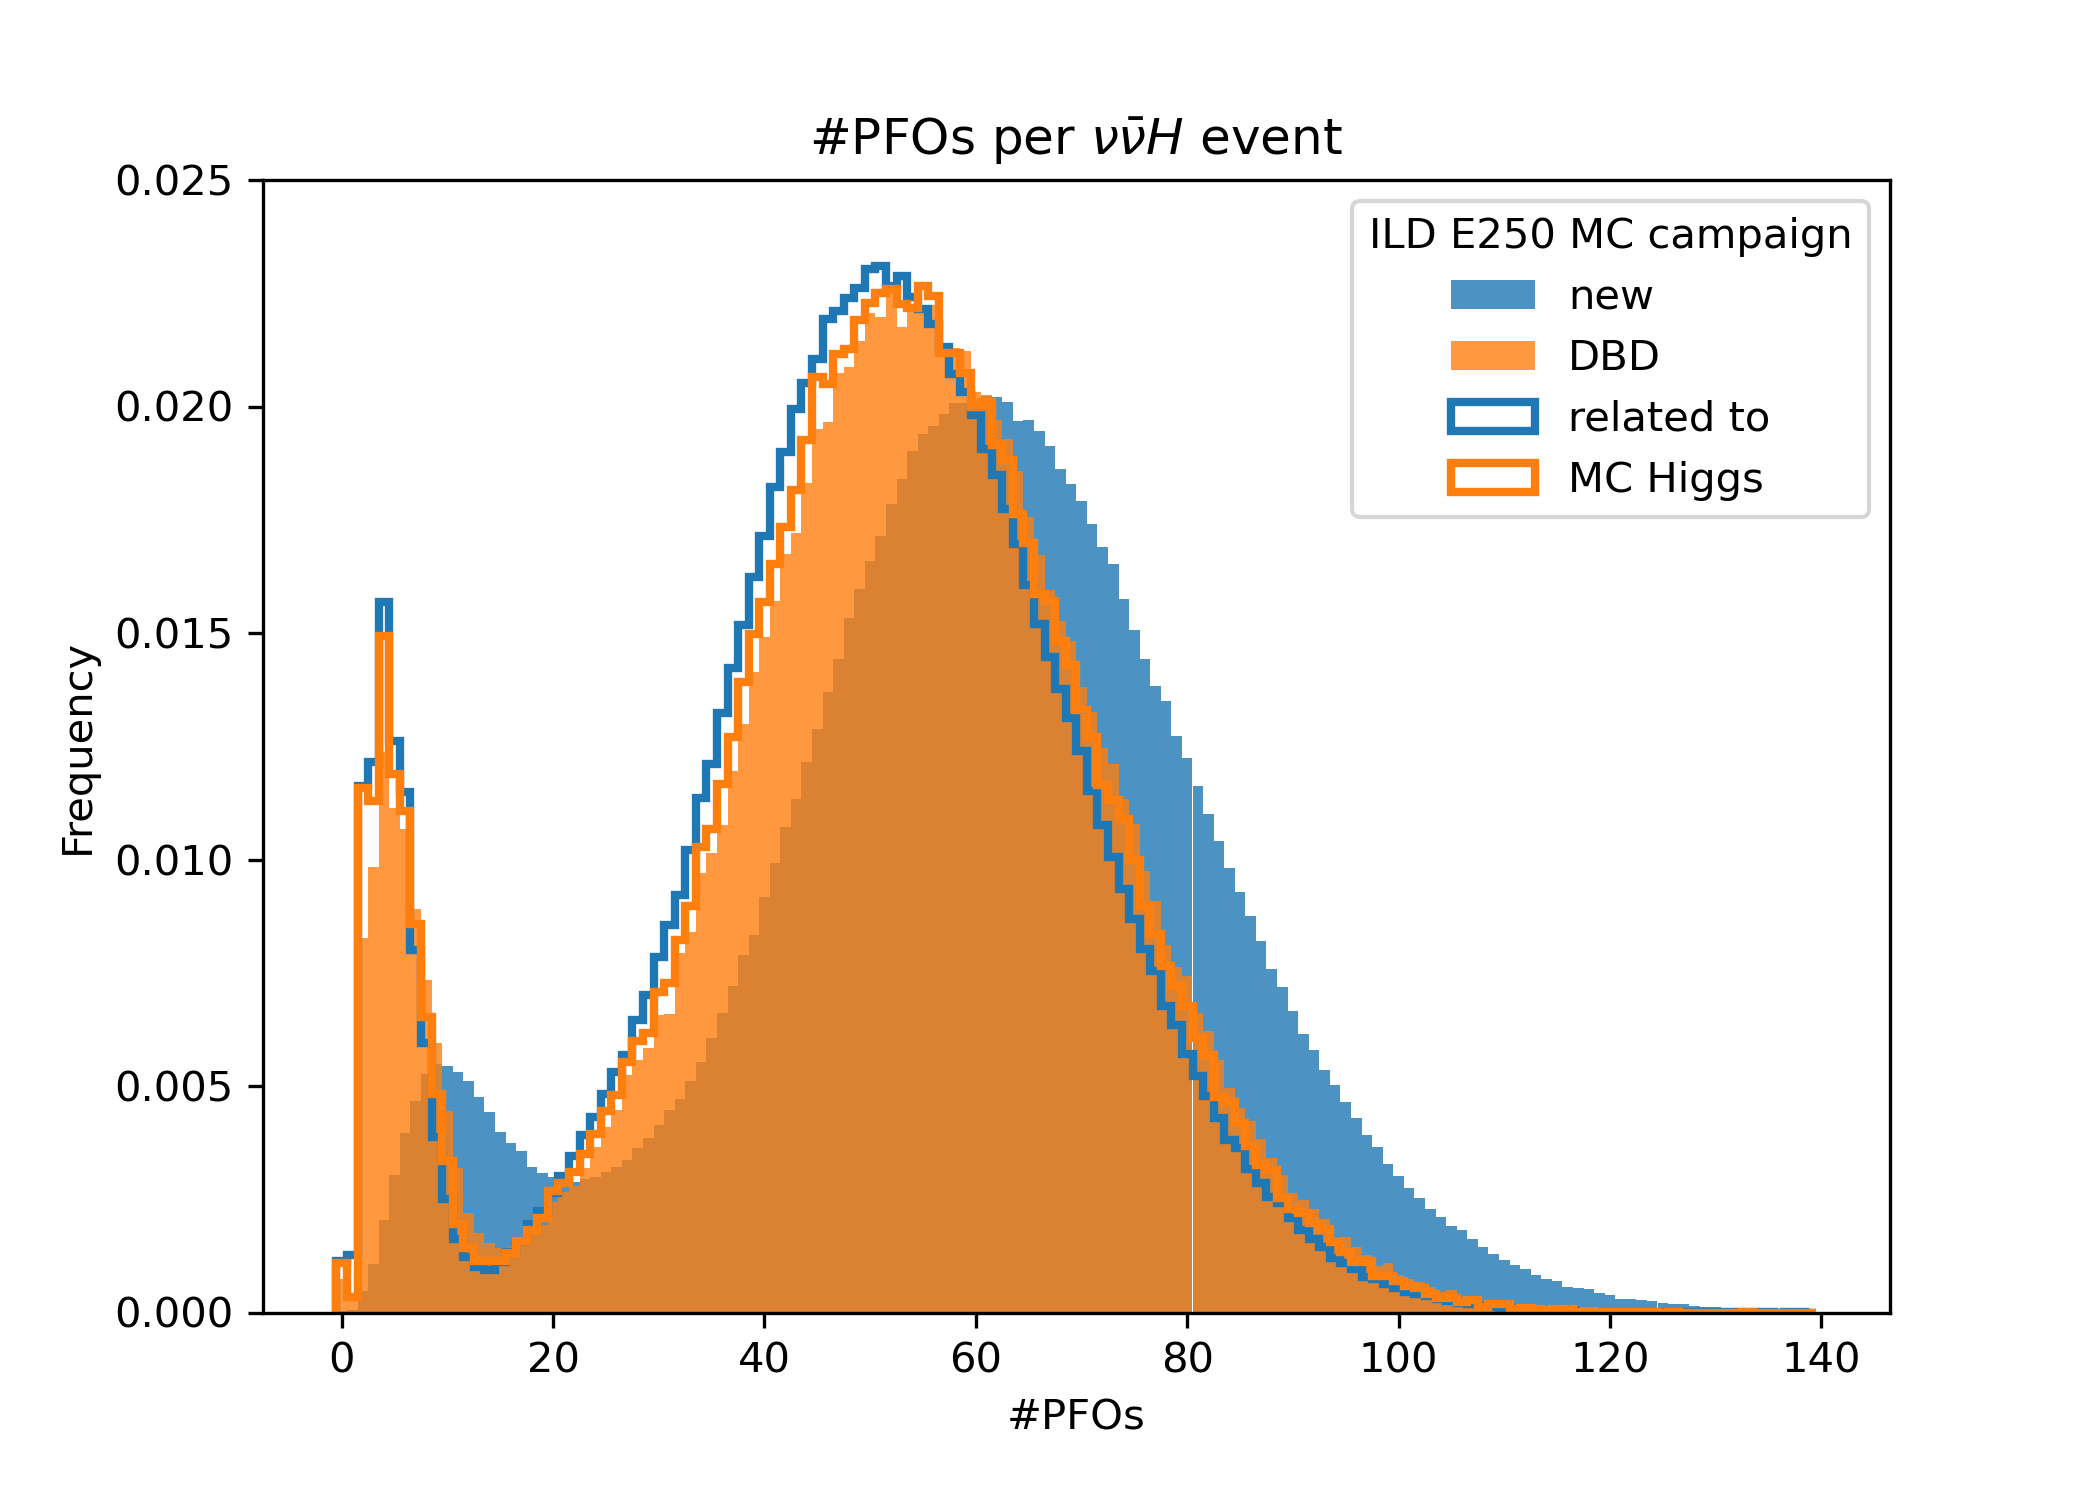
\includegraphics[height=0.8\textheight, width=\textwidth, keepaspectratio]
      {n_pfos_full_and_only_higgs}}
      \only<2->{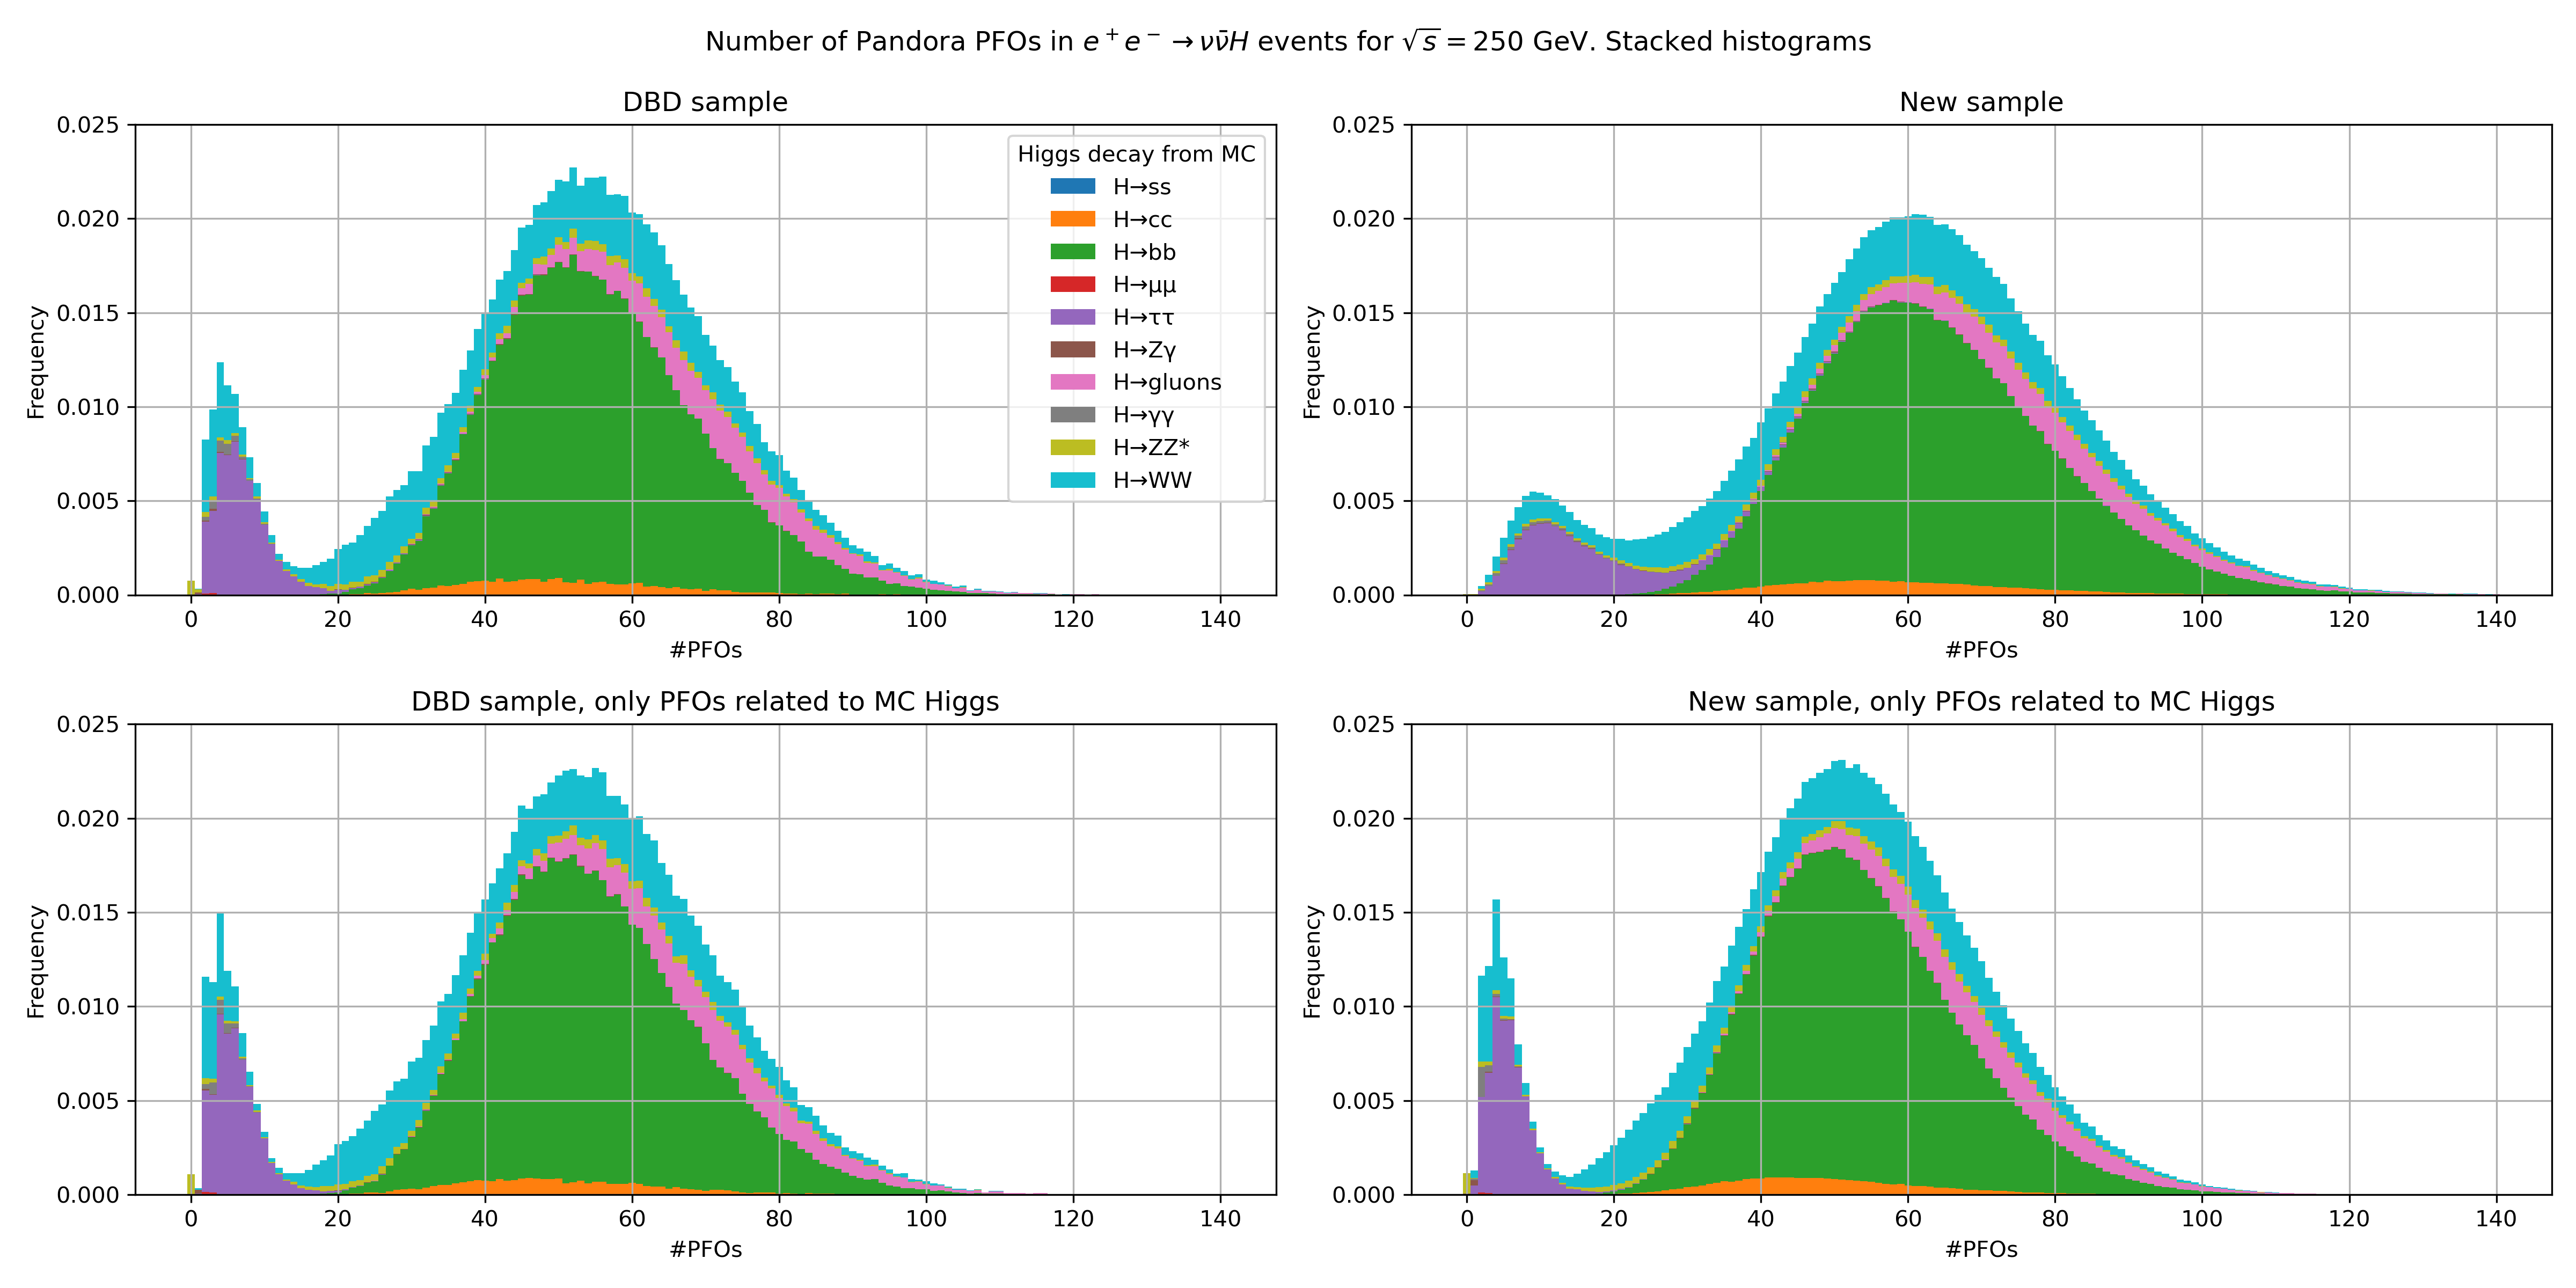
\includegraphics[height=0.8\textheight, width=\textwidth, keepaspectratio]
        {decays_stacked_n_pfos}}
  \end{center}
  \end{frame}